% 第 7 章 变量替换与形式的积分
\chapter{变量替换与形式的积分}

积分是数学中最基本的概念之一. 在微积分中，你首先学会在 $\mathbb{R}$ 上积分一元函数. 然后，你学会在 $\mathbb{R}^2$ 和 $\mathbb{R}^3$ 上积分二元和三元函数. 在此之后，你学会在变量替换之后积分函数，最后在向量微积分中你学会沿曲线积分向量场并在曲面上积分向量场. 事实证明，微分形式实际上是积分的好对象. 事实上，微分形式的积分与你在微积分中学到的\newterm{change-of-variables}{变量替换}{change of variables}公式之间有着密切的关系. 在第 1 节中，我们用 Riemann 和来定义 $\mathbb{R}^2$ 上 2-形式的积分. $\mathbb{R}^n$ 上 $n$-形式的积分可以类似地定义. 然后我们利用第 6 章的思想与 Riemann 和过程，从第一原理推导出变量替换公式. 在第 2 节中，我们仔细考察一个简单的变量替换例子. 第 3 节继续考察从笛卡尔坐标到极坐标、柱坐标和球坐标的变换. 最后，在第 4 节中我们考虑一个更一般的设置，在那里我们看看如何在参数化的一维和二维曲面上积分任意的 1-形式和 2-形式.

\section{微分形式的积分}

我们首先考察以 Riemann 和为基础的积分的基本定义. 我们将从求函数图像下方的体积开始，这基本上就是你在微积分中见过的. 目前我们假定欧几里得流形 $\mathbb{R}^2$ 上使用传统的笛卡尔坐标. 设 $R$ 是平面上的一个区域，设 $f(x,y)$ 是我们求其图像下方体积的函数. 在微积分课上你应该记得以下步骤：
\begin{enumerate}
  \item 选择一组覆盖区域 $R$ 的等间距格点 $\{x_i\}_{i=1}^{n}$ 和 $\{y_j\}_{j=1}^{m}$. 这组格点给出点 $(x_i,y_j)\in\mathbb{R}^2_{xy}$.
  \item 令 $\Delta x_i=x_{i+1}-x_i$，$\Delta y_j=y_{j+1}-y_j$.
  \item 对每个 $i=1,\ldots,n$ 和 $j=1,\ldots,m$，求 $f(x_i,y_j)\Delta x_i\Delta y_j$.
  \item 对 $i$ 和 $j$ 求和：$\sum_i\sum_j f(x_i,y_j)\Delta x_i\Delta y_j$.
  \item 取这个二重和当 $n,m\to\infty$ 时的极限，即当 $\Delta x_i,\Delta y_j\to 0$ 时的极限，并将其定义为 $\iint_R f(x,y)\,dx\,dy$.
\end{enumerate}
本质上，我们是在用乘积 $f(x_i,y_j)\Delta x_i\Delta y_j$ 来近似 $f(x,y)$ 图像下方、矩形 $\Delta x_i\Delta y_j$ 上方的体积，见图~\ref{fig:7-1} 与图~\ref{fig:7-2}. 当然，这只是理论定义，我们并不是这样实际计算积分的，我们有你在微积分中学到的一整套积分技术可以使用.

\begin{figure}[htbp]
  \centering
  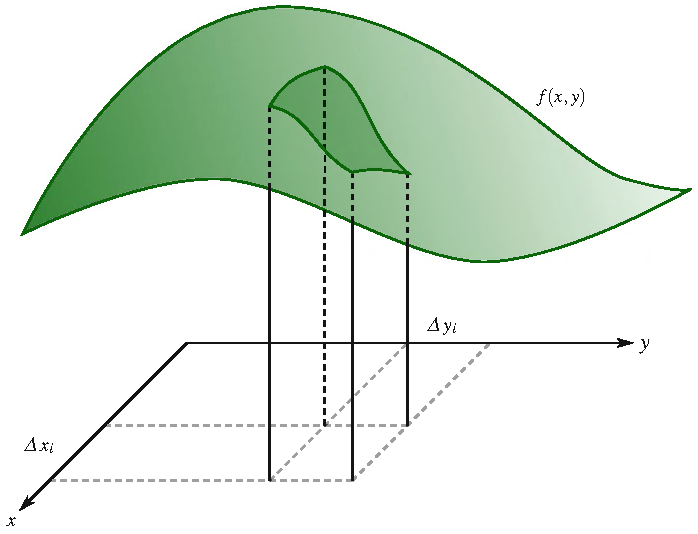
\includegraphics[width=0.827\linewidth]{images/vector/fig-7-1.pdf}
  \caption{$f(x,y)$ 图像下方、矩形 $\Delta x_i\Delta y_j$ 上方的体积}
  \label{fig:7-1}
\end{figure}

\begin{figure}[htbp]
  \centering
  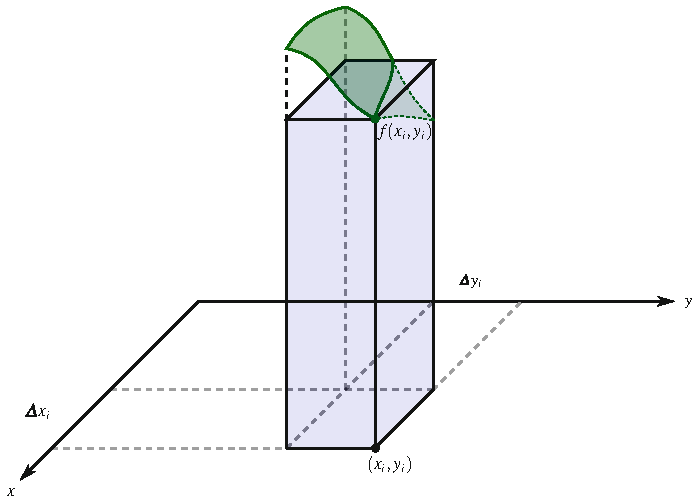
\includegraphics[width=0.827\linewidth]{images/vector/fig-7-2.pdf}
  \caption{$f(x,y)$ 图像下方、矩形 $\Delta x_i\Delta y_j$ 上方的近似体积，由乘积 $f(x_i,y_j)\Delta x_i\Delta y_j$ 给出，以蓝色显示}
  \label{fig:7-2}
\end{figure}

现在，我们基本上将以一种更适合微分形式情形的方式，同时复制上面的思想与过程，从而给出微分形式 $\alpha=f(x,y)\,dx\wedge dy$ 在区域 $R\subset\mathbb{R}^2$ 上积分的理论定义. 不过我们要提醒，这里给出的确切过程隐含地依赖于我们仍然处于欧几里得流形 $\mathbb{R}^2$ 这一事实. 对 $\mathbb{R}^n$ 的更一般定义当然是可能的，但它要求更加注意记号，而那会掩盖基本思想.

\begin{enumerate}
  \item 选择一组覆盖区域 $R$ 的等间距格点 $\{x_i\}_{i=1}^{n}$ 和 $\{y_j\}_{j=1}^{m}$. 这组格点给出点 $(x_i,y_j)\in\mathbb{R}^2_{xy}$.
  \item 对每个 $i,j$ 定义向量
  \[
  V^1_{i,j}=\binom{x_{i+1}-x_i}{0}_{(x_i,y_j)},\qquad
  V^2_{i,j}=\binom{0}{y_{j+1}-y_j}_{(x_i,y_j)}.
  \]
  注意，我们可以把向量 $V^1_{i,j}$ 和 $V^2_{i,j}$ 看作切空间 $T_{(x_i,y_j)}\mathbb{R}^2$ 的元素. 见图~\ref{fig:7-3}. 这里我们隐式地假定我们处于欧几里得情形，可以作出这一等同. 于是我们得到类似图~\ref{fig:7-4} 的情形.
  \item 对每个 $i,j$，计算 $f(x_i,y_j)\,dx\wedge dy\bigl(V^1_{i,j},V^2_{i,j}\bigr)$.
  \item 对 $i$ 和 $j$ 求和：$\sum_i\sum_j f(x_i,y_j)\,dx\wedge dy\bigl(V^1_{i,j},V^2_{i,j}\bigr)$.
  \item 取这个二重和当 $m,n\to\infty$ 时的极限，即当 $|x_{i+1}-x_i|,|y_{j+1}-y_j|\to 0$ 时的极限，并将其定义为 $\iint_R f\,dx\wedge dy$. 也就是说，
  \[
  \iint_R f\,dx\wedge dy\equiv\lim_{m,n\to\infty}\sum_{i=1}^{n}\sum_{j=1}^{m}f(x_i,y_j)\,dx\wedge dy\bigl(V^1_{i,j},V^2_{i,j}\bigr).
  \]
\end{enumerate}

\begin{figure}[htbp]
  \centering
  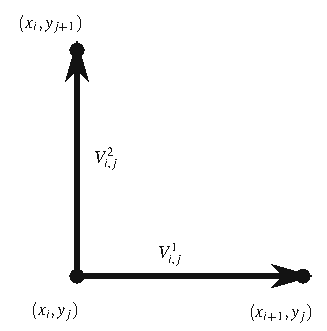
\includegraphics[width=0.481\linewidth]{images/vector/fig-7-3.pdf}
  \caption{向量 $V^1_{i,j}$ 与 $V^2_{i,j}$. 尽管它们的定义方式如此，我们还是可以把 $V^1_{i,j},V^2_{i,j}$ 视为 $T_{(x_i,y_j)}\mathbb{R}^2$ 的元素}
  \label{fig:7-3}
\end{figure}

\begin{figure}[htbp]
  \centering
  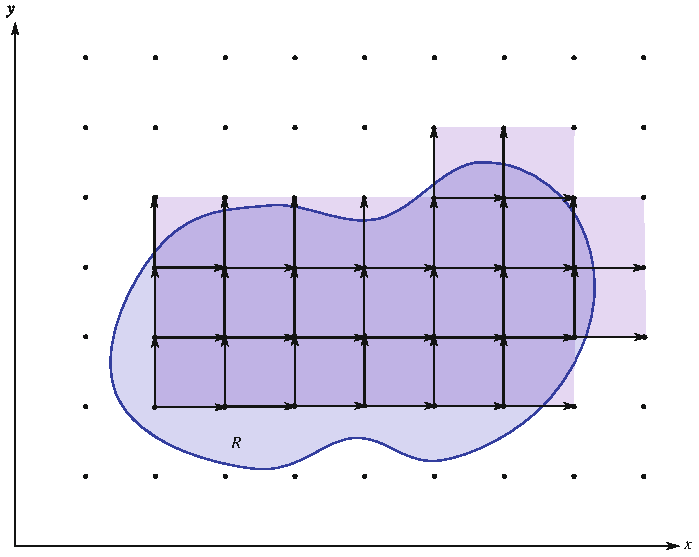
\includegraphics[width=0.829\linewidth]{images/vector/fig-7-4.pdf}
  \caption{区域 $R\subset\mathbb{R}^2$，连同覆盖它的等间距格点 $\{x_i\}_{i=1}^{n}$、$\{y_j\}_{j=1}^{m}$，以及区域 $R$ 中每个点的向量 $V^1_{i,j}$ 与 $V^2_{i,j}$. 当格点靠得越来越近，即当 $|x_{i+1}-x_i|,|y_{j+1}-y_j|\to 0$ 时，区域 $R$ 被越来越精确地近似}
  \label{fig:7-4}
\end{figure}

请比较并对照这两个过程. 它们本质上是一样的，除了求面积的方式. 在第一个过程的第 2 步中，我们只是求出数 $\Delta x_i$ 和 $\Delta y_j$，而在第二个过程中我们求出向量 $V^1_{i,j}$ 和 $V^2_{i,j}$. 然后，在第一个过程的第 3 步中，我们只是通过求乘积 $\Delta x_i\Delta y_j$ 来求流形中矩形的面积，而在第二个过程中我们用面积形式 $dx\wedge dy$ 和向量 $V^1_{i,j},V^2_{i,j}$ 来求面积，即我们求出 $dx\wedge dy\bigl(V^1_{i,j},V^2_{i,j}\bigr)$. 本质上，这就是两个过程之间仅有的差别. 但请注意，在第一个过程中我们定义的积分是 $\iint_R f(x,y)\,dx\,dy$，而在第二个过程中我们定义的积分是 $\iint_R f(x,y)\,dx\wedge dy$. 正因为如此，人们有时会把微分形式 $f(x,y)\,dx\wedge dy$ 的积分直接定义为
\[
\iint_R f(x,y)\,dx\wedge dy\equiv\iint_R f(x,y)\,dx\,dy,
\]
而不是按第二个过程用 Riemann 和来定义. 这里唯一的问题是，第一个过程及其相关的积分 $\iint_R f(x,y)\,dx\,dy$ 不记录定向，而第二个过程及其相关的积分 $\iint_R f(x,y)\,dx\wedge dy$ 记录\newterm{orientation}{定向}{orientation}.

\begin{question}\label{q:7-1}
以上面五步为指导，用 Riemann 和定义微分形式
\[
\alpha=f(x_1,x_2,\ldots,x_n)\,dx_1\wedge dx_2\wedge\cdots\wedge dx_n
\]
在区域 $R\subset\mathbb{R}^n$ 上的积分.
\end{question}

现在，假定我们发现求积分 $\int_R f(x_1,\ldots,x_n)\,dx_1\wedge\cdots\wedge dx_n$，或者等价地求积分 $\int_R f(x_1,\ldots,x_n)\,dx_1\cdots dx_n$，是困难的，但我们注意到，通过做一次适当的变量替换它会变得容易，
\[
\mathbb{R}^n_{x_1x_2\cdots x_n}\xrightarrow{\ \varphi\ }\mathbb{R}^n_{\varphi_1\varphi_2\cdots\varphi_n},\qquad(x_1,x_2,\ldots,x_n)\longmapsto(\varphi_1,\varphi_2,\ldots,\varphi_n).
\]
我们想在微分形式的语境下，从第一原理，即从 Riemann 和的定义，推导出这个变量替换公式. 换言之，我们要证明
\[
\int_R f\,dx_1\wedge\cdots\wedge dx_n=\int_{\varphi(R)}f\circ\varphi^{-1}\,T^*\varphi^{-1}\cdot\bigl(dx_1\wedge\cdots\wedge dx_n\bigr).
\]
通过做变量替换 $\varphi$，我们把 $R\subset\mathbb{R}^n_{x_1x_2\cdots x_n}$ 映到 $\varphi(R)\subset\mathbb{R}^n_{\varphi_1\varphi_2\cdots\varphi_n}$. 我们还需要假定 $\varphi$ 有逆 $\varphi^{-1}$.

\begin{enumerate}
  \item 在 $\mathbb{R}^n_{x_1x_2\cdots x_n}$ 上选择一组格点 $\{(x_{i_1},\ldots,x_{i_n})\}$. 这又给出新坐标系 $\mathbb{R}^n_{\varphi_1\varphi_2\cdots\varphi_n}$ 中的一组格点
  \[
  \Bigl\{\bigl(\varphi_1(x_{i_1},\ldots,x_{i_n}),\ldots,\varphi_n(x_{i_1},\ldots,x_{i_n})\bigr)\Bigr\}=\{(\varphi_1,\ldots,\varphi_n)\},
  \]
  见图~\ref{fig:7-5}.

  \begin{figure}[htbp]
    \centering
    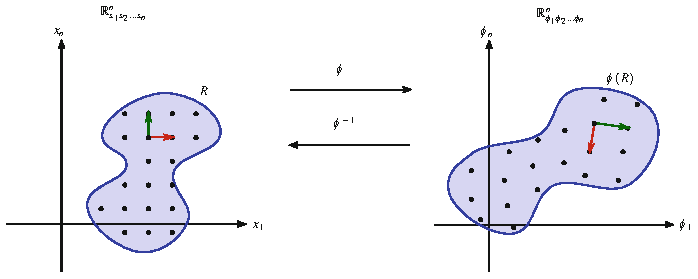
\includegraphics[width=0.960\linewidth]{images/vector/fig-7-5.pdf}
    \caption{$\mathbb{R}^n_{x_1x_2\cdots x_n}$ 中的格点 $\{(x_{i_1},\ldots,x_{i_n})\}$ 产生 $\mathbb{R}^n_{\varphi_1\varphi_2\cdots\varphi_n}$ 中的格点 $\{(\varphi_1,\ldots,\varphi_n)\}$. 图中显示了两个向量的前推}
    \label{fig:7-5}
  \end{figure}

  \item 对每个 $i_1,\ldots,i_n$ 定义向量
  \[
  V^1_{i_1\cdots i_n}=\begin{bmatrix}x_{i_1+1}-x_{i_1}\\0\\\vdots\\0\end{bmatrix}_{(x_{i_1},x_{i_2},\ldots,x_{i_n})},\quad\cdots\quad
  V^n_{i_1\cdots i_n}=\begin{bmatrix}0\\\vdots\\0\\x_{i_n+1}-x_{i_n}\end{bmatrix}_{(x_{i_1},x_{i_2},\ldots,x_{i_n})}.
  \]
  注意，由于流形是一个与切空间同构的向量空间，我们可以断言向量
\[
V^1_{i_1\cdots i_n},\ldots,V^n_{i_1\cdots i_n}\in T_{(x_{i_1},\ldots,x_{i_n})}\mathbb{R}^n_{x_1\cdots x_n}.
\]
由向量 $V^1_{i_1\cdots i_n},\ldots,V^n_{i_1\cdots i_n}$ 张成的平行六面体的体积由
  \[
  dx_1\wedge\cdots\wedge dx_n\bigl(V^1_{i_1\cdots i_n},\ldots,V^n_{i_1\cdots i_n}\bigr)
  \]
  给出.
  \item 位于 $n$ 维平行六面体上方、$f$ 图像下方的 $(n+1)$ 维体积由
  \[
  f(x_{i_1},\ldots,x_{i_n})\,dx_1\wedge\cdots\wedge dx_n\bigl(V^1_{i_1\cdots i_n},\ldots,V^n_{i_1\cdots i_n}\bigr)
  \]
  近似. 接下来，在每个格点 $p=\{(x_{i_1},\ldots,x_{i_n})\}\in\mathbb{R}^n_{x_1\cdots x_n}$ 处，该点的向量 $V^1_{i_1\cdots i_n},\ldots,V^n_{i_1\cdots i_n}$ 的前推为
  \[
  T_p\varphi\cdot V^1_{i_1\cdots i_n},\ldots,T_p\varphi\cdot V^n_{i_1\cdots i_n}\in T_{\varphi(p)}\mathbb{R}^n_{\varphi_1\varphi_2\cdots\varphi_n}.
  \]
  另外注意，对每个 $i$，有 $T\varphi^{-1}\cdot T\varphi\cdot V^i_{i_1\cdots i_n}=V^i_{i_1\cdots i_n}$，所以按定义我们有
  \begin{align*}
  &T^*\varphi^{-1}\cdot\bigl(dx_1\wedge\cdots\wedge dx_n\bigr)\\
  &\qquad\qquad\qquad\Bigl(T\varphi\cdot V^1_{i_1\cdots i_n},\ldots,T\varphi\cdot V^n_{i_1\cdots i_n}\Bigr)\\
  &=dx_1\wedge\cdots\wedge dx_n\Bigl(T\varphi^{-1}\cdot T\varphi\cdot V^1_{i_1\cdots i_n},\\
  &\qquad\qquad\qquad\qquad\ldots,T\varphi^{-1}\cdot T\varphi\cdot V^n_{i_1\cdots i_n}\Bigr)\\
  &=dx_1\wedge\cdots\wedge dx_n\Bigl(V^1_{i_1\cdots i_n},\ldots,V^n_{i_1\cdots i_n}\Bigr).
  \end{align*}
  接着，我们注意到 $f(x_{i_1},\ldots,x_{i_n})=f\circ\varphi^{-1}\circ\varphi(x_{i_1},\ldots,x_{i_n})$. 把这两者结合起来，我们有
  \begin{align*}
  &f(x_{i_1},\ldots,x_{i_n})\,dx_1\wedge\cdots\wedge dx_n\Bigl(V^1_{i_1\cdots i_n},\ldots,V^n_{i_1\cdots i_n}\Bigr)\\
  &=f\circ\varphi^{-1}\circ\varphi(x_{i_1},\ldots,x_{i_n})\,T^*\varphi^{-1}\cdot\bigl(dx_1\wedge\cdots\wedge dx_n\bigr)\Bigl(T\varphi\cdot V^1_{i_1\cdots i_n},\ldots,T\varphi\cdot V^n_{i_1\cdots i_n}\Bigr)\\
  &=f\circ\varphi^{-1}(\varphi_1,\ldots,\varphi_n)\,T^*\varphi^{-1}\cdot\bigl(dx_1\wedge\cdots\wedge dx_n\bigr)\Bigl(T\varphi\cdot V^1_{i_1\cdots i_n},\ldots,T\varphi\cdot V^n_{i_1\cdots i_n}\Bigr).
  \end{align*}
  注意，在上面最后一个等式中我们写
  \[
  \varphi(x_{i_1},\ldots,x_{i_n})=\Bigl(\varphi_1(x_{i_1},\ldots,x_{i_n}),\ldots,\varphi_n(x_{i_1},\ldots,x_{i_n})\Bigr)=(\varphi_1,\ldots,\varphi_n).
  \]
  \item 现在我们对所有 $i_1,\ldots,i_n$ 求和，得到
  \begin{align*}
  &\sum_{i_1,\ldots,i_n}f(x_{i_1},\ldots,x_{i_n})\,dx_1\wedge\cdots\wedge dx_n\Bigl(V^1_{i_1\cdots i_n},\ldots,V^n_{i_1\cdots i_n}\Bigr)\\
  &=\sum_{i_1,\ldots,i_n}f\circ\varphi^{-1}(\varphi_1,\ldots,\varphi_n)\,T^*\varphi^{-1}\bigl(dx_1\wedge\cdots\wedge dx_n\bigr)\Bigl(T\varphi\cdot V^1_{i_1\cdots i_n},\ldots,T\varphi\cdot V^n_{i_1\cdots i_n}\Bigr).
  \end{align*}
  \item 取当 $|x_{i_j+1}-x_{i_j}|\to 0$（$j=1,\ldots,n$）时的极限，我们定义
  \[
  \begin{aligned}
  \int_R f(x_1,\ldots,x_n)\,dx_1\wedge\cdots\wedge dx_n
  &=\lim_{|x_{i_j+1}-x_{i_j}|\to 0}\sum_{i_1,\ldots,i_n}f(x_{i_1},\ldots,x_{i_n})\,dx_1\wedge\cdots\wedge dx_n\\
  &\qquad\qquad\qquad\qquad\qquad\Bigl(V^1_{i_1\cdots i_n},\ldots,V^n_{i_1\cdots i_n}\Bigr)
  \end{aligned}
  \]
  以及
  \[
  \begin{aligned}
  \int_{\varphi(R)}f\circ\varphi^{-1}(\varphi_1,\ldots,\varphi_n)\,T^*\varphi^{-1}
  &=\lim_{|x_{i_j+1}-x_{i_j}|\to 0}\sum_{i_1,\ldots,i_n}f\circ\varphi^{-1}(\varphi_1,\ldots,\varphi_n)\\
  &\qquad\qquad T^*\varphi^{-1}\cdot\bigl(dx_1\wedge\cdots\wedge dx_n\bigr)\Bigl(T\varphi\cdot V^1_{i_1\cdots i_n},\\
  &\qquad\qquad\qquad\qquad\ldots,T\varphi\cdot V^n_{i_1\cdots i_n}\Bigr).
  \end{aligned}
  \]
  把第 (4) 步与这些定义结合起来，就给出下面的等式：
  \[
  \begin{aligned}
  \text{变量替换公式}\\
  &\int_R f(x_1,\ldots,x_n)\,dx_1\wedge\cdots\wedge dx_n\\
  &=\int_{\varphi(R)}f\circ\varphi^{-1}(\varphi_1,\ldots,\varphi_n)\\
  &\qquad\qquad\qquad\qquad\cdot T^*\varphi^{-1}\bigl(dx_1\wedge\cdots\wedge dx_n\bigr).
  \end{aligned}
  \]
\end{enumerate}

让我们更仔细地考察这个等式. 左边相当直接：积分在 $x_1\cdots x_n$-坐标中进行，我们在区域 $R$ 上用与 $x_1\cdots x_n$-坐标相联系的体积形式 $dx_1\wedge\cdots\wedge dx_n$ 积分函数 $f(x_1,\ldots,x_n)$. 现在，让我们拆开这个等式的右边. 首先，我们有坐标变换 $\varphi:\mathbb{R}^n\to\mathbb{R}^n$，
\begin{align*}
\mathbb{R}^n_{x_1x_2\cdots x_n}\xrightarrow{\ \varphi\ }\mathbb{R}^n_{\varphi_1\varphi_2\cdots\varphi_n}, \\
(x_1,x_2,\ldots,x_n)\longmapsto(\varphi_1,\varphi_2,\ldots,\varphi_n),
\end{align*}
它给出图~\ref{fig:7-6} 中的图像. 我们在 $\mathbb{R}^n_{x_1x_2\cdots x_n}$ 中积分的区域是 $R$，我们在 $\mathbb{R}^n_{\varphi_1\varphi_2\cdots\varphi_n}$ 中积分的区域是它的像 $\varphi(R)$. 函数 $f:\mathbb{R}^n\to\mathbb{R}$ 是变量 $x_1,x_2,\ldots,x_n$ 的函数，而函数 $f\circ\varphi^{-1}:\mathbb{R}^n\to\mathbb{R}$ 是变量 $\varphi_1,\varphi_2,\ldots,\varphi_n$ 的函数. 最后，$dx_1\wedge\cdots\wedge dx_n$ 是 $\mathbb{R}^n_{x_1x_2\cdots x_n}$ 上的面积形式. 但请注意，右边的形式是 $T^*\varphi^{-1}\cdot\bigl(dx_1\wedge\cdots\wedge dx_n\bigr)$，即面积形式 $dx_1\wedge\cdots\wedge dx_n$ 由 $\varphi^{-1}$ 的\newterm{pull-back}{拉回}{pull-back}，而不是面积形式 $d\varphi_1\wedge\cdots\wedge d\varphi_n$. 在做变量替换时，这是本质的一点.

\begin{figure}[htbp]
  \centering
  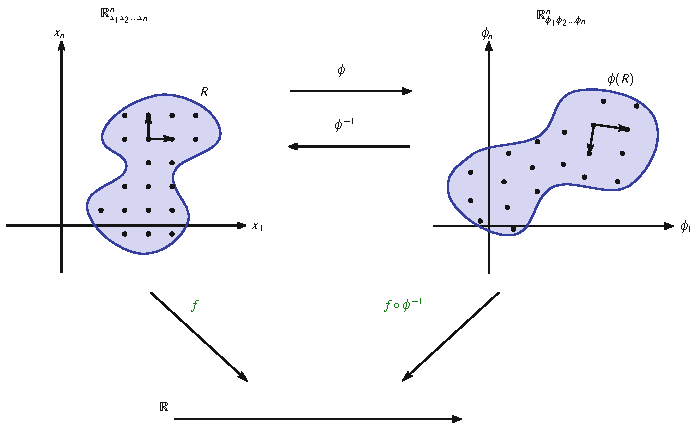
\includegraphics[width=0.960\linewidth]{images/vector/fig-7-6.pdf}
  \caption{当我们做变量替换时，必须改变积分中的三样东西：区域（蓝色）、函数（绿色）和体积形式（红色）. 左边的向量被 $T\varphi$ 前推到右边的向量}
  \label{fig:7-6}
\end{figure}

现在还有最后一个问题需要我们简要提及. 无论你是否上过入门分析课程、是否见过 Fubini 定理的证明，或者之前是否听说过 Fubini 定理，你无疑都知道它的结论. 假定我们有一个矩形区域 $R=\{a\leq x\leq b,\ c\leq y\leq d\}$ 和一个连续函数 $f:R\to\mathbb{R}$，那么 Fubini 定理断言
\[
\int_a^b\int_c^d f(x,y)\,dy\,dx=\int_c^d\int_a^b f(x,y)\,dx\,dy.
\]
它基本上是说我们可以交换积分顺序. 这实际上要求我们的函数 $f$ 在某种意义上是``好的''. 我们不想在这里深入技术细节（把它留给你分析课程），只需说你要处理的大部分函数事实上都是``好的''. 然而，在微分形式的语境下，我们当然有 $dx\wedge dy=-dy\wedge dx$，所以我们会有
\[
\int_a^b\int_c^d f(x,y)\,dy\wedge dx=-\int_c^d\int_a^b f(x,y)\,dx\wedge dy,
\]
除非你也同时改变矩形 $R$ 的定向. 这个问题以后还会再次出现，但我们不会在上面花太多时间. 一般而言，用微分形式积分会考虑定向，而微积分中是不考虑的. 因此，你的答案可能会相差一个符号.

\section{一个简单的例子}

现在，我们通过考察一个使用与第 6.1 节中相同的坐标变换的简单例子，来应用我们刚刚所做的，看看体积形式在变量替换的积分中所扮演的角色. 我们首先在 $\mathbb{R}^2_{xy}$ 的一个给定区域上积分一个函数. 然后我们应用变量替换公式，在 $\mathbb{R}^2_{uv}$ 上完成积分. 我们还将隐式地使用下面的等同：
\[
\iint_R f(x,y)\,dx\,dy\equiv\iint_R f(x,y)\,dx\wedge dy.
\]
假定我们想在由直线 $x=0$、$y=0$ 和 $y=x-2$ 围成的 $\mathbb{R}^2$ 中的区域上积分函数 $f(x,y)=x$，如图~\ref{fig:7-7} 所示. 我们首先关于 $x$ 积分，然后关于 $y$ 积分，
\begin{align*}
\int_{-2}^{0}\int_{y+2}^{0}x\,dx\,dy
&=\int_{-2}^{0}\left.\frac{x^2}{2}\right|_{y+2}^{0}dy\\
&=\int_{-2}^{0}\frac{-(y+2)^2}{2}\,dy\\
&=\int_{-2}^{0}-\frac{y^2+4y+4}{2}\,dy\\
&=-\left.\left(\frac{y^3}{6}+y^2+2y\right)\right|_{-2}^{0}\\
&=-\frac{4}{3}.
\end{align*}

\begin{figure}[htbp]
  \centering
  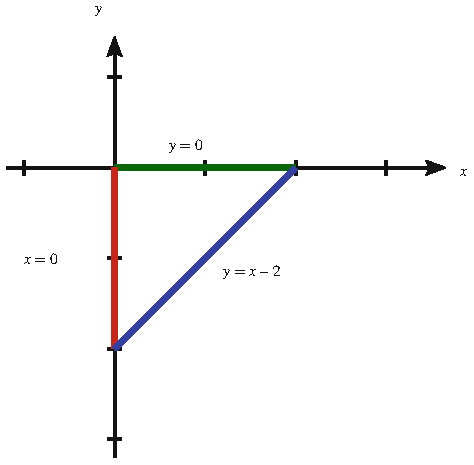
\includegraphics[width=0.568\linewidth]{images/vector/fig-7-7.pdf}
  \caption{由直线 $x=0$、$y=0$ 和 $y=x-2$ 围成的 $\mathbb{R}^2$ 中的区域.}
  \label{fig:7-7}
\end{figure}

现在我们要做同一个积分，只不过在不同坐标中. 为此我们必须利用我们在第 7.1 节中推导出的变量替换公式，
\[
\int_R f(x_1,\ldots,x_n)\,dx_1\wedge\cdots\wedge dx_n=\int_{\varphi(R)}f\circ\varphi^{-1}(\varphi_1,\ldots,\varphi_n)\,T^*\varphi^{-1}\cdot\bigl(dx_1\wedge\cdots\wedge dx_n\bigr).
\]
对我们的具体例子而言，一般的变量替换公式简化为
\[
\iint_R f(x,y)\,dx\wedge dy=\iint_{\varphi(R)}f\circ\varphi^{-1}(u,v)\,T^*\varphi^{-1}\cdot(dx\wedge dy).
\]
所有这一切归结为：当我们做变量替换时，必须改变积分中的三样东西——区域（蓝色）、函数（绿色）和体积形式（红色）. 见图~\ref{fig:7-8}.

\begin{figure}[htbp]
  \centering
  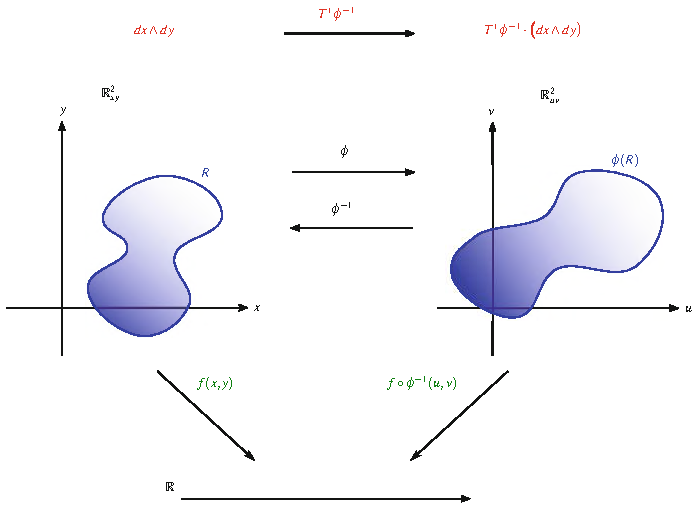
\includegraphics[width=0.948\linewidth]{images/vector/fig-7-8.pdf}
  \caption{当我们做变量替换时，必须改变积分中的三样东西：区域（蓝色）、函数（绿色）和体积形式（红色）}
  \label{fig:7-8}
\end{figure}

回到我们的例子，我们将变量替换为由 $u=x+y$ 和 $v=x-y$ 定义的 $uv$-坐标系. 换言之，我们将使用坐标变换 $\varphi:\mathbb{R}^2_{xy}\to\mathbb{R}^2_{uv}$，它由 $\varphi(x,y)=\bigl(u(x,y),v(x,y)\bigr)=(x+y,x-y)$ 给出. 我们逐一考虑需要改变的三样东西. 首先考虑我们在 $\mathbb{R}^2_{uv}$ 中积分的区域. 坐标变换 $u=x+y$ 和 $v=x-y$ 可以改写为 $x=\frac{u+v}{2}$，$y=\frac{u-v}{2}$，这意味着在变换下，定义边界的方程变为
\begin{align*}
x=0&\Rightarrow u=-v,\\
y=0&\Rightarrow u=v,\\
y=x-2&\Rightarrow v=2.
\end{align*}
于是我们的区域在 $\mathbb{R}^2_{uv}$ 中的像如图~\ref{fig:7-9} 所示.

\begin{figure}[htbp]
  \centering
  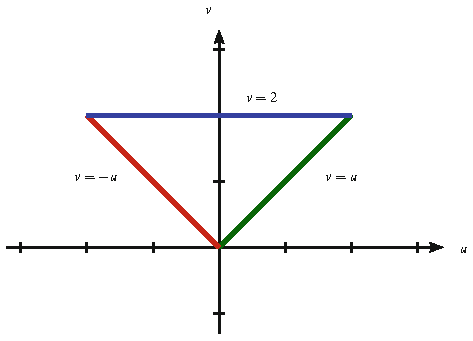
\includegraphics[width=0.599\linewidth]{images/vector/fig-7-9.pdf}
  \caption{图~\ref{fig:7-7} 中的区域在变换 $\varphi(x,y)=\bigl(u(x,y),v(x,y)\bigr)=(x+y,x-y)$ 下于 $\mathbb{R}^2_{uv}$ 中的像}
  \label{fig:7-9}
\end{figure}

其次，我们考虑函数. 我们要积分的函数 $f(x,y)=x$ 变换为 $f\circ\varphi^{-1}(u,v)=\frac{u+v}{2}$. 第三，我们需要考虑体积形式如何变化. 回想映射 $\varphi^{-1}$ 诱导拉回映射 $T^*\varphi^{-1}$，
\begin{align*}
\mathbb{R}^2_{uv}\xrightarrow{\ \varphi^{-1}\ }\mathbb{R}^2_{xy},\qquad(u,v)\longmapsto(x,y),\qquad
T^*\varphi^{-1}:\Lambda^2\bigl(\mathbb{R}^2_{xy}\bigr)\xleftarrow{\ }\Lambda^2\bigl(\mathbb{R}^2_{uv}\bigr), \\
T^*\varphi^{-1}\cdot dx\wedge dy\longmapsto dx\wedge dy.
\end{align*}
在第 6 章中我们已经求得
\[
T^*\varphi^{-1}\cdot\bigl(dx\wedge dy\bigr)=-\frac{1}{2}\,du\wedge dv.
\]

\begin{figure}[htbp]
  \centering
  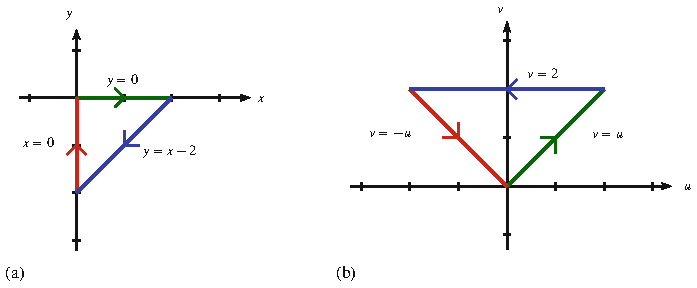
\includegraphics[width=0.909\linewidth]{images/vector/fig-7-10.pdf}
  \caption{映射 $\varphi:\mathbb{R}^2_{xy}\to\mathbb{R}^2_{uv}$（$\varphi(x,y)=\bigl(u(x,y),v(x,y)\bigr)=(x+y,x-y)$）对我们要积分的区域的影响. (a) $\mathbb{R}^2_{xy}$ 中包围的面积为 $2$，定向为顺时针. (b) $\mathbb{R}^2_{uv}$ 中包围的面积为 $4$，定向为逆时针}
  \label{fig:7-10}
\end{figure}

在变换 $\varphi$ 下，区域的各个角按如下方式映射：
\[
\begin{array}{c}
\mathbb{R}^2_{xy}\xrightarrow{\ \varphi\ }\mathbb{R}^2_{uv}\\
(x,y)\longmapsto(x+y,x-y)\equiv(u,v)\\
(0,0)\longmapsto(0,0)\\
(2,0)\longmapsto(2,2)\\
(0,-2)\longmapsto(-2,2).
\end{array}
\]
于是我们可以看出，当我们沿区域绕行时，$\mathbb{R}^2_{uv}$ 中的定向与 $\mathbb{R}^2_{xy}$ 中的定向是不同的. 另外，请比较图~\ref{fig:7-10} 中两个区域的面积. 这张图清楚地说明了为什么我们需要使用面积形式的拉回. 在变量替换下，我们要积分的区域的面积和定向都会改变. 通过使用面积形式的拉回，我们补偿了这些变化. 微分形式，特别是体积形式，随身携带着我们做积分问题的变量替换所需的信息.

总之，$\iint_R x\,dx\,dy$ 确实应该被想成 $\iint_R x\,dx\wedge dy$. 当我们改变坐标时，区域 $R=\{(x,y)\,|\,0\leq x\leq 2,\ x-2\leq y\leq 0\}$ 变成 $\widetilde{R}=\{(u,v)\,|\,0\leq v\leq 2,\ -v\leq u\leq v\}$，$f(x,y)=x$ 变成 $\widetilde{f}(u,v)=\frac{u+v}{2}$，而 $dx\,dy$——它实际上是 $dx\wedge dy$——变成 $-\frac{1}{2}\,du\wedge dv$，或者 $-\frac{1}{2}\,du\,dv$. 换言之，我们有
\[
\iint_R f(x,y)\,dx\,dy=\iint_{\widetilde{R}}\widetilde{f}(u,v)\left(-\frac{1}{2}\right)du\,dv,
\]
这实际上是
\[
\iint_R f(x,y)\,dx\wedge dy=\iint_{\widetilde{R}}\widetilde{f}(u,v)\left(-\frac{1}{2}\right)du\wedge dv.
\]
现在让我们在变换后的区域上积分变换后的函数，
\begin{align*}
\int_0^2\int_{-v}^{v}\frac{u+v}{2}\left(-\frac{1}{2}\right)du\,dv
&=\int_0^2\left.\left(-\frac{1}{2}\right)\left(\frac{u^2}{4}+\frac{uv}{2}\right)\right|_{-v}^{v}dv\\
&=\left(-\frac{1}{2}\right)\int_0^2 v^2\,dv\\
&=\left(-\frac{1}{2}\right)\left.\frac{v^3}{3}\right|_0^2\\
&=\left(-\frac{1}{2}\right)\frac{8}{3}\\
&=-\frac{4}{3}.
\end{align*}
通常，变量替换（也称为换基）会使我们要积分的函数简单得多，从而使积分更容易. 为了看一个例子，假定我们想在和之前相同的区域 $R=\{(x,y)\,|\,0\leq x\leq 2,\ x-2\leq y\leq 0\}$ 上积分 $f(x,y)=e^{\frac{x+y}{x-y}}$. 希望简化这个函数、从而简化积分的愿望，正是选择新坐标 $u=x+y$ 和 $v=x-y$ 的动机，
\begin{align*}
\int_{-2}^{0}\int_{y+2}^{0}e^{\frac{x+y}{x-y}}dx\,dy
&=\int_{-2}^{0}\int_{y+2}^{0}e^{\frac{x+y}{x-y}}dx\wedge dy\\
&=\int_0^2\int_{-v}^{v}e^{\frac{u}{v}}\left(-\frac{1}{2}\right)du\wedge dv\\
&=\int_0^2\int_{-v}^{v}e^{\frac{u}{v}}\left(-\frac{1}{2}\right)du\,dv\\
&=\left(-\frac{1}{2}\right)\int_0^2\left.\left[ve^{\frac{u}{v}}\right]\right|_{-v}^{v}dv\\
&=\left(-\frac{1}{2}\right)\int_0^2 v\left(e^{\frac{v}{v}}-e^{-\frac{v}{v}}\right)dv\\
&=\left(-\frac{1}{2}\right)\left(e^1-e^{-1}\right)\int_0^2 v\,dv\\
&=\left(-\frac{1}{2}\right)\left(e^1-e^{-1}\right)\left.\frac{v^2}{2}\right|_0^2\\
&=-\left(e^1-e^{-1}\right)\\
&\approx-2.35.
\end{align*}
显然，对所有 $x$ 和 $y$ 都有 $e^{\frac{x+y}{x-y}}>0$，所以你是在一个你通常认为是正的区域上积分一个正的函数，因此你很自然地期望得到一个正的体积，而不是负的. 当然，以这种方式思考时，我们没有考虑空间的``定向''. 但人们自然期望体积为正这一事实，正是经典微积分课程中对多余的那一项——Jacobian，在这里是 $-\frac{1}{2}$——取绝对值的原因. 本质上这相当于约定：无论坐标变换过程中发生了什么，我们总是假定我们的坐标轴遵循``右手法则''.

然而，当我们开始处理更高级、更抽象的数学时，我们希望能够记录流形的定向，而这正是微分形式所做的. 回想一下，微分形式记录定向这一事实全部源于我们的楔积是用行列式定义的，而行列式本身——按照我们展开它的方式——记录定向. 在我们的例子中出现负号，是因为当我们用变换把两个向量从 $xy$ 平面前推到 $uv$ 平面时，像向量改变了``手性''，因此正定向的区域变成负定向的区域，反之亦然.

\section{极坐标、柱坐标与球坐标}

现在我们将考察一系列涉及极坐标、柱坐标和球坐标的例子. 尽管你在微积分中见过这些坐标系，这里的讲述将把你已经知道的东西与微分形式的视角联系起来.

\subsection{极坐标例子}

现在，让我们动手处理一个涉及极坐标的实际例子. 假定我们想求由 $z=0$ 平面和抛物面 $z=3-x^2-y^2$ 围成的三维立体的体积，见图~\ref{fig:7-11}. 首先我们求抛物面与 $z=0$ 平面的交线，
\[
z=0\Rightarrow 0=3-x^2-y^2\Rightarrow x^2+y^2=3,
\]
它给出 $xy$ 平面中的区域 $R=\{x^2+y^2\leq 3\}$. 于是我们要计算的积分是
\[
\int_R 3-x^2-y^2\,dx\wedge dy,
\]
或者用更传统的微积分记号，
\[
\int_{-\sqrt{3}}^{\sqrt{3}}\int_{-\sqrt{3-y^2}}^{\sqrt{3-y^2}}\bigl(3-x^2-y^2\bigr)dx\,dy.
\]
毫无疑问，这个计算会是很麻烦的.

\begin{figure}[htbp]
  \centering
  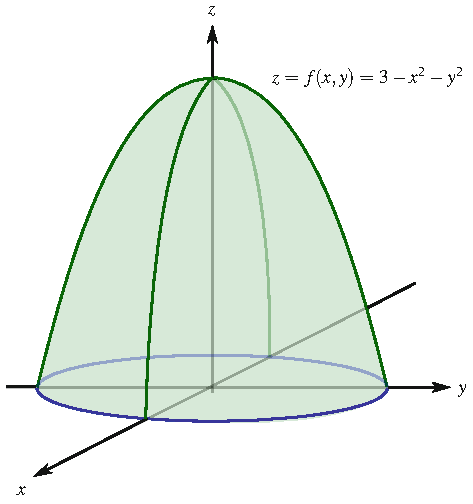
\includegraphics[width=0.561\linewidth]{images/vector/fig-7-11.pdf}
  \caption{由 $z=0$ 平面和抛物面 $z=3-x^2-y^2$ 围成的三维立体}
  \label{fig:7-11}
\end{figure}

\begin{question}\label{q:7-2}
尝试用你在微积分课上记得的技术完成这个积分，不做变量替换，看看你能进行到哪一步.
\end{question}

当我们实际计算积分时，在矩形区域上积分显然比其他形状的区域上积分简单得多. 由于这个区域是 $xy$ 平面中的一个圆盘，使用极坐标变换会在 $r\theta$-平面中产生一个矩形区域. 也就是说，给定极坐标变换
\[
x=r\cos\theta,\qquad y=r\sin\theta,
\]
这个区域在极坐标变换下的像是
\[
\varphi(R)=\{0\leq r\leq\sqrt{3},\ 0\leq\theta\leq 2\pi\},
\]
如图~\ref{fig:7-12} 所示.

\begin{figure}[htbp]
  \centering
  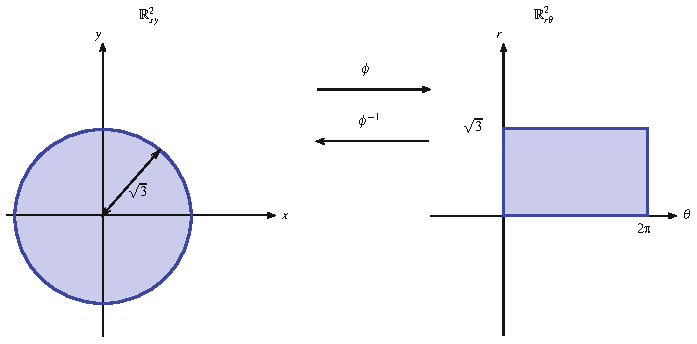
\includegraphics[width=0.907\linewidth]{images/vector/fig-7-12.pdf}
  \caption{圆形区域 $\{x^2+y^2\leq 3\}$ 在极坐标变换下的像是矩形区域 $\{0\leq r\leq\sqrt{3},\ 0\leq\theta\leq 2\pi\}$}
  \label{fig:7-12}
\end{figure}

\begin{question}\label{q:7-3}
证明区域 $\varphi(R)$ 确实是 $\{0\leq r\leq\sqrt{3},\ 0\leq\theta\leq 2\pi\}$.
\end{question}

于是我们要利用上一节从第一原理推导出的等式，用坐标变换来简化我们的积分，
\[
\int_R f\,dx_1\wedge\cdots\wedge dx_n=\int_{\varphi(R)}f\circ\varphi^{-1}\,T^*\varphi^{-1}\cdot\bigl(dx_1\wedge\cdots\wedge dx_n\bigr).
\]
在这里我们花一点时间，就我们使用的记号以及 $xy$-平面与 $r\theta$-平面的比较谈几点. 第一，微积分教材中通常给出的极坐标变换 $x=r\cos\theta$、$y=r\sin\theta$，是从 $r\theta$-平面到 $xy$-平面的变换，而不是反过来. 从 $xy$-平面到 $r\theta$-平面的变换由相当复杂的
\[
r=\sqrt{x^2+y^2},\qquad\theta=\arctan\frac{y}{x}
\]
给出. 我们还需要把 $r\theta$-平面限制在 $0<\theta<2\pi$，以便 $\arctan$ 有定义. 我们将对此稍稍放宽要求，但对我们的积分问题来说这样做不会带来麻烦. 另外，我们把哪个方向标记为 $\varphi$、哪个标记为 $\varphi^{-1}$ 当然完全是任意的，但为了与上一节的记号保持一致，我们把从 $xy$-平面到 $r\theta$-平面的变换标记为 $\varphi$，把逆变换标记为 $\varphi^{-1}$. 想一想这有点令人惊讶，但事实上拥有 $\varphi^{-1}$，即用 $r$ 和 $\theta$ 表示的 $x$ 和 $y$，使我们能轻易地求出 $\varphi(R)$ 和 $f\circ\varphi^{-1}$，
\begin{align*}
f\circ\varphi^{-1}&=3-(r\cos\theta)^2-(r\sin\theta)^2\\
&=3-r^2(\sin^2\theta+\cos^2\theta)\\
&=3-r^2.
\end{align*}
最后，我们求 $T^*\varphi^{-1}\cdot\bigl(dx\wedge dy\bigr)$. 为此我们首先注意到 $T^*\varphi^{-1}\cdot\bigl(dx\wedge dy\bigr)$ 具有某个函数 $g$ 决定的 $g(r,\theta)\,d\theta\wedge dr$ 的形式. 接着我们注意到
\begin{align*}
g(r,\theta)&=g(r,\theta)\,d\theta\wedge dr\left(\binom{1}{0},\binom{0}{1}\right)\\
&=T^*\varphi^{-1}\cdot\bigl(dx\wedge dy\bigr)\left(\binom{1}{0},\binom{0}{1}\right)\\
&=dx\wedge dy\left(T\varphi^{-1}\cdot\binom{1}{0},T\varphi^{-1}\cdot\binom{0}{1}\right).
\end{align*}
为了继续下去，我们现在需要求 $T\varphi^{-1}$，
\[
T\varphi^{-1}=\begin{bmatrix}\frac{\partial x}{\partial\theta}&\frac{\partial x}{\partial r}\\\frac{\partial y}{\partial\theta}&\frac{\partial y}{\partial r}\end{bmatrix}=\begin{bmatrix}-r\sin\theta&\cos\theta\\r\cos\theta&\sin\theta\end{bmatrix},
\]
于是我们可以计算
\begin{align*}
T\varphi^{-1}\cdot\binom{1}{0}=\begin{bmatrix}-r\sin\theta&\cos\theta\\r\cos\theta&\sin\theta\end{bmatrix}\binom{1}{0}=\binom{-r\sin\theta}{r\cos\theta}, \\
T\varphi^{-1}\cdot\binom{0}{1}=\begin{bmatrix}-r\sin\theta&\cos\theta\\r\cos\theta&\sin\theta\end{bmatrix}\binom{0}{1}=\binom{\cos\theta}{\sin\theta},
\end{align*}
这反过来给出
\begin{align*}
dx\wedge dy\left(T\varphi^{-1}\cdot\binom{1}{0},T\varphi^{-1}\cdot\binom{0}{1}\right)
&=dx\wedge dy\left(\binom{-r\sin\theta}{r\cos\theta},\binom{\cos\theta}{\sin\theta}\right)\\
&=\begin{vmatrix}-r\sin\theta&\cos\theta\\r\cos\theta&\sin\theta\end{vmatrix}\\
&=-r\sin^2\theta-r\cos^2\theta\\
&=-r,
\end{align*}
这意味着 $g(r,\theta)=-r$. 因此
\[
T^*\varphi^{-1}\cdot\bigl(dx\wedge dy\bigr)=-r\,d\theta\wedge dr.
\]
我们当然已经在上一章中求得了这一结果.

现在我们有了把积分改写为极坐标所需的全部要素. 当然，我们费了很大的劲，把每一步都事无巨细地展示出来. 一旦你这样做了几次，最终结果就现成可用，你可以直接把积分写成极坐标形式，
\begin{align*}
\int_{-\sqrt{3}}^{\sqrt{3}}\int_{-\sqrt{3-y^2}}^{\sqrt{3-y^2}}\bigl(3-x^2-y^2\bigr)dx\,dy
&=\int_R f\,dx\wedge dy\\
&=\int_{\varphi(R)}f\circ\varphi^{-1}\,T^*\varphi^{-1}\cdot(dx\wedge dy)\\
&=\int_0^{\sqrt{3}}\int_0^{2\pi}(3-r^2)(-r)\,d\theta\wedge dr\\
&=\int_0^{\sqrt{3}}\int_0^{2\pi}-3r+r^3\,d\theta\,dr.
\end{align*}
这是一个比我们一开始的那个容易得多的积分. 唯一需要注意的是面积形式 $dx\wedge dy$ 的拉回中 $r$ 前面的负号，它反映了定向的改变.

\begin{question}\label{q:7-4}
完成这个积分. 如果你设法完成了问题~\ref{q:7-2} 中的积分，答案是否相同？
\end{question}

\subsection{柱坐标例子}

现在我们将做一个积分问题，其中变量替换为柱坐标会使积分更容易. 假定我们想在由圆锥面 $z=\sqrt{x^2+y^2}$ 和平面 $z=2$ 围成的区域上积分函数 $f(x,y)=x^2+y^2$. 换言之，我们想求积分
\[
\int_R (x^2+y^2)\,dx\,dy\,dz.
\]
为了精确地画出表示这个积分的图形，我们需要四个维度，所以我们不打算那样做. 只需想象一幅类似图~\ref{fig:7-1} 的漫画. 用笛卡尔坐标写出区域 $R$ 的一种方式是
\[
R=\Bigl\{(x,y,z)\,\Bigl|\,-2\leq x\leq 2,\ -\sqrt{4-x^2}\leq y\leq\sqrt{4-x^2},\ \sqrt{x^2+y^2}\leq z\leq 2\Bigr\},
\]
它给出积分
\[
\int_{-2}^{2}\int_{-\sqrt{4-x^2}}^{\sqrt{4-x^2}}\int_{\sqrt{x^2+y^2}}^{2}(x^2+y^2)\,dz\,dy\,dx.
\]
然而，和之前一样，我们可以看出做这个积分会相当复杂.

\begin{question}\label{q:7-5}
证明由圆锥面 $z=\sqrt{x^2+y^2}$ 和平面 $z=2$ 围成的区域确实可以写成
\[
\Bigl\{-2\leq x\leq 2,\ -\sqrt{4-x^2}\leq y\leq\sqrt{4-x^2},\ \sqrt{x^2+y^2}\leq z\leq 2\Bigr\}.
\]
\end{question}

\begin{question}\label{q:7-6}
尝试用你在微积分课上记得的技术完成这个计算，不做变量替换，看看你能进行到哪一步.
\end{question}

但是当我们考虑柱坐标变换
\[
\mathbb{R}^3_{r\theta z}\xrightarrow{\ \varphi^{-1}\ }\mathbb{R}^3_{xyz},\qquad(r,\theta,z)\longmapsto(r\cos\theta,r\sin\theta,z),
\]
很明显，这个区域用柱坐标描述要简单得多，
\[
\varphi(R)=\{0\leq\theta\leq 2\pi,\ 0\leq r\leq 2,\ r\leq z\leq 2\}.
\]

\begin{figure}[htbp]
  \centering
  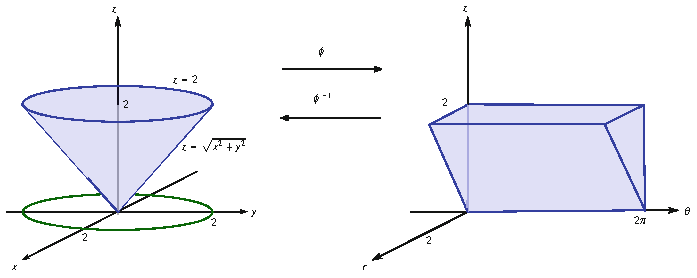
\includegraphics[width=0.960\linewidth]{images/vector/fig-7-13.pdf}
  \caption{映射 $\varphi:\mathbb{R}^3_{xyz}\to\mathbb{R}^3_{r\theta z}$ 对我们要积分的区域的影响}
  \label{fig:7-13}
\end{figure}

\begin{question}\label{q:7-7}
证明区域 $\varphi(R)$ 确实是 $\{0\leq\theta\leq 2\pi,\ 0\leq r\leq 2,\ r\leq z\leq 2\}$.
\end{question}

我们要指出，为了与上一节的记号保持一致，我们把从 $\mathbb{R}^3_{r\theta z}$ 到 $\mathbb{R}^3_{xyz}$ 的映射记为 $\varphi^{-1}$，而不是像上一章那样记为 $\varphi$. 只要我们限制映射在 $\mathbb{R}^3_{r\theta z}$ 的适当定义域上，使我们的逆有定义，那么这应该不会引起混淆. 见图~\ref{fig:7-13}. 我们还有 $f\circ\varphi^{-1}=r^2$，以及 $T^*\varphi^{-1}\cdot(dx\wedge dy\wedge dz)=-r\,d\theta\wedge dr\wedge dz$.

\begin{question}\label{q:7-8}
求出 $f\circ\varphi^{-1}$ 和 $T^*\varphi^{-1}\cdot(dx\wedge dy\wedge dz)$.
\end{question}

最后，利用上一节推导出的恒等式，我们得到
\begin{align*}
\int_R f\,dx\wedge dy\wedge dz
&=\int_{\varphi(R)}f\circ\varphi^{-1}\,T^*\varphi^{-1}\cdot\bigl(dx\wedge dy\wedge dz\bigr)\\
&=\int_{\varphi(R)}(r^2)(-r)\,d\theta\wedge dr\wedge dz\\
&=\int_{\varphi(R)}(r^2)\,r\,d\theta\wedge dz\wedge dr\\
&=\int_0^{2\pi}\int_0^2\int_r^2 r^3\,d\theta\,dz\,dr.
\end{align*}

\begin{question}\label{q:7-9}
完成这个积分.
\end{question}

\subsection{球坐标例子}

我们用一个使用球坐标的坐标变换例子来结束本节. 假定我们想在整个单位球
\[
R=\bigl\{x^2+y^2+z^2\leq 1\bigr\}
\]
上积分函数 $f(x,y,z)=e^{(x^2+y^2+z^2)^{3/2}}$. 一个能完成这件事的积分是
\[
\int_{-1}^{1}\int_{-\sqrt{1-x^2}}^{\sqrt{1-x^2}}\int_{-\sqrt{1-x^2-y^2}}^{\sqrt{1-x^2-y^2}}e^{(x^2+y^2+z^2)^{3/2}}\,dz\,dy\,dx,
\]

\begin{figure}[htbp]
  \centering
  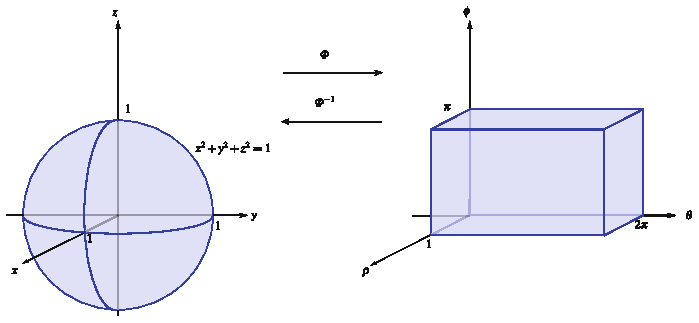
\includegraphics[width=0.960\linewidth]{images/vector/fig-7-14.pdf}
  \caption{映射 $\Phi:\mathbb{R}^3_{xyz}\to\mathbb{R}^3_{\rho\theta\varphi}$ 对我们要积分的区域的影响}
  \label{fig:7-14}
\end{figure}

它充其量显然会是很难的. 在球坐标变换
\[
\mathbb{R}^3_{\rho\theta\varphi}\xrightarrow{\ \Phi^{-1}\ }\mathbb{R}^3_{xyz},\qquad(\rho,\theta,\varphi)\longmapsto(\rho\sin\varphi\cos\theta,\rho\sin\varphi\sin\theta,\rho\cos\varphi)
\]
下，我们的区域变成
\[
\Phi(R)=\{0\leq\rho\leq 1,\ 0\leq\theta\leq 2\pi,\ 0\leq\varphi\leq\pi\}.
\]
由于 $\varphi$ 是球坐标中使用的标准变量之一，我们把映射记为大写的 $\Phi$. 见图~\ref{fig:7-14}.

\begin{question}\label{q:7-10}
证明区域 $\Phi(R)$ 确实是 $\{0\leq\rho\leq 1,\ 0\leq\theta\leq 2\pi,\ 0\leq\varphi\leq\pi\}$.
\end{question}

我们还得到 $f\circ\Phi^{-1}=e^{(\rho^2)^{3/2}}=e^{\rho^3}$，以及 $T^*\Phi^{-1}\cdot(dx\wedge dy\wedge dz)=-\rho^2\sin\varphi\,d\rho\wedge d\theta\wedge d\varphi$. 同样，利用上一节推导出的恒等式，我们有
\begin{align*}
\int_R f\,dx\wedge dy\wedge dz
&=\int_{\Phi(R)}f\circ\Phi^{-1}\,T^*\Phi^{-1}\cdot\bigl(dx\wedge dy\wedge dz\bigr)\\
&=\int_{\Phi(R)}(e^{\rho^3})(-\rho^2\sin\varphi)\,d\rho\wedge d\theta\wedge d\varphi\\
&=\int_0^{\pi}\int_0^{2\pi}\int_0^1-\rho^2e^{\rho^3}\sin\varphi\,d\rho\,d\theta\,d\varphi.
\end{align*}

\begin{question}\label{q:7-11}
完成这个积分.
\end{question}

\section{参数化曲面上微分形式的积分}

到目前为止，我们考察了一种特定类型的积分问题，即我们要积分的区域在其他某个坐标系中有更简单表示的问题. 然而，还有一些其他类型的积分问题我们可以用微分形式来做.

只要在一个 $n$ 维流形上有一个 $n$-形式，我们就可以对它积分. 例如，我们可以在曲线上积分 1-形式，在曲面上积分 2-形式，在三维空间中积分 3-形式，等等. 只要我们有流形 $\Sigma_k\subset\mathbb{R}^n$（$k<n$）的一个\newterm{parametrization}{参数化}{parametrization}，即一个可逆映射 $\varphi^{-1}:U\subset\mathbb{R}^k\to\Sigma_k\subset\mathbb{R}^n$，我们就可以用 $T^*\varphi^{-1}$ 把 $k$-形式拉回到 $U\subset\mathbb{R}^k$，并在那里积分，从而在 $\Sigma_k$ 上积分 $k$-形式. 用 $\varphi^{-1}$ 而不是 $\varphi$ 来命名参数化有点不寻常，但我们想保持与上一章一致的记号. 本节的其余部分将讨论在 $\mathbb{R}^n$ 中以参数化曲面 $\Sigma_k$ 给出的子流形上积分形式. 我们之前推导出的等式是
\[
\int_R f\,dx_1\wedge\cdots\wedge dx_n=\int_{\varphi(R)}f\circ\varphi^{-1}\,T^*\varphi^{-1}\cdot\bigl(dx_1\wedge\cdots\wedge dx_n\bigr).
\]
我们通常想使用的这个等式的形式是
\[
\text{$k$ 维参数化曲面 $\Sigma_k$ 上 $k$-形式的积分}\qquad\int_{\Sigma_k}\alpha=\int_{\varphi(\Sigma_k)}T^*\varphi^{-1}\cdot\alpha.
\]
当 $k=1$ 时，我们得到一条曲线，我们经常写 $\Sigma_1=C$.

\begin{question}\label{q:7-12}
用与第 7.1 节类似的涉及 Riemann 和的论证来定义这个公式.
\end{question}

但在那之前，我们还想重申：你可以——而且经常确实——积分各种各样不是微分形式的对象. 例如，要求 $\mathbb{R}^3$ 中二维曲面的表面积，你需要积分
\[
\sqrt{(dx\wedge dy)^2+(dy\wedge dz)^2+(dz\wedge dx)^2},
\]
这不是一个微分形式，因为它不是多重线性的，尽管它是由微分形式 $dx\wedge dy$、$dy\wedge dz$ 和 $dz\wedge dx$ 组成的. 然而，对于简单的曲面，有时这样的积分仍然可以手工完成. 否则，一般可以用数值方法求出数值答案. 形式之所以如此有用，原因之一就是广义 Stokes 定理. 不过，广义 Stokes 定理并不适用于不是形式的被积函数.

\subsection{线积分}

这里我们将考察一些涉及在一维流形上积分 1-形式的例子. 我们将利用恒等式
\[
\int_C\alpha=\int_{\varphi(C)}T^*\varphi^{-1}\cdot\alpha.
\]

\textbf{例一.} 我们从 $\mathbb{R}^2$ 中的一个例子开始. 我们将沿两条不同的曲线积分 1-形式 $y^2dx+xdy$. 第一条曲线 $C_1$ 是从 $(-5,-3)$ 到 $(0,2)$ 的线段. 第二条曲线 $C_2$ 是抛物线 $x=4-y^2$ 从 $(-5,-3)$ 到 $(0,2)$ 的弧. 我们首先计算沿 $C_1$ 的积分. 为此，我们首先要做的就是把路径 $C_1$ 参数化为 $\varphi^{-1}(t)=\bigl(x(t),y(t)\bigr)=(5t-5,5t-3)$. 令 $R=[0,1]\subset\mathbb{R}$，我们有 $\varphi^{-1}(R)=\bigl\{(x,y)\,\bigl|\,x=5t-5,\ y=5t-3,\ 0\leq t\leq 1\bigr\}=C_1$. 见图~\ref{fig:7-15}. 利用映射 $\varphi^{-1}$，我们求 $T\varphi^{-1}$，
\[
T\varphi^{-1}=\begin{bmatrix}\frac{\partial x}{\partial t}\\\frac{\partial y}{\partial t}\end{bmatrix}=\binom{5}{5},
\]
于是我们得到诱导的切映射和余切映射，
\begin{align*}
T_p(\mathbb{R})\xrightarrow{\;T\varphi^{-1}\;}T_{\varphi^{-1}(p)}\bigl(\mathbb{R}^2\bigr),\qquad[1]\in T_p(\mathbb{R})\longmapsto T\varphi^{-1}\cdot[1]=\binom{5}{5}[1]=\binom{5}{5}\in T_{\varphi^{-1}(p)}\bigl(\mathbb{R}^2\bigr), \\
T^*_p(\mathbb{R})\xleftarrow{\;T^*\varphi^{-1}\;}T^*_{\varphi^{-1}(p)}\bigl(\mathbb{R}^2\bigr),\qquad f(t)\,dt=T^*\varphi^{-1}\cdot\bigl(y^2dx+xdy\bigr)\longmapsto y^2dx+xdy,
\end{align*}
其中 $f(t)$ 是某个函数. 这个关于 $t$ 的函数正是我们想求的. 注意 $f(t)\,dt\bigl([1]\bigr)=f(t)$，所以我们有
\begin{align*}
f(t)&=f(t)\,dt\bigl([1]\bigr)\\
&=T^*\varphi^{-1}\cdot\bigl(y^2dx+xdy\bigr)\bigl([1]\bigr)\\
&=\bigl(y^2dx+xdy\bigr)\bigl(T\varphi^{-1}\cdot[1]\bigr)\\
&=\bigl(y^2dx+xdy\bigr)\binom{5}{5}\\
&=y^2dx\binom{5}{5}+xdy\binom{5}{5}\\
&=y^2(5)+x(5)\\
&=(5t-3)^2(5)+(5t-5)(5)\\
&=125t^2-125t+20,
\end{align*}
所以我们有
\[
T^*\varphi^{-1}\cdot\bigl(y^2dx+xdy\bigr)=(125t^2-125t+20)\,dt.
\]
利用下面的等式
\[
\int_C\alpha=\int_{\varphi(C)}T^*\varphi^{-1}\cdot\alpha,
\]
我们的积分变成
\begin{align*}
\int_{C_1}y^2dx+xdy
&=\int_{[0,1]}\bigl(125t^2-125t+20\bigr)dt\\
&=\int_0^1\bigl(125t^2-125t+20\bigr)dt\\
&=-\frac{5}{6}.
\end{align*}

\begin{figure}[htbp]
  \centering
  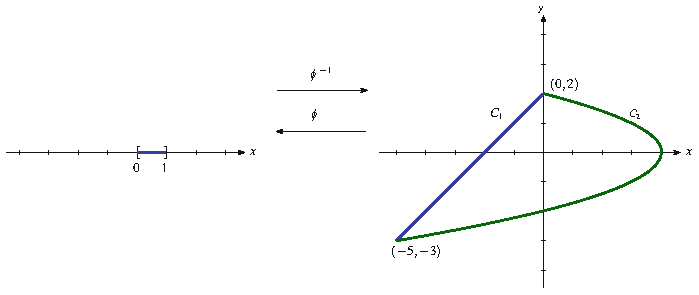
\includegraphics[width=0.960\linewidth]{images/vector/fig-7-15.pdf}
  \caption{映射 $\varphi^{-1}$ 把 $[0,1]$ 送到曲线 $C_1$}
  \label{fig:7-15}
\end{figure}

现在我们将沿第二条路径 $C_2$ 求 1-形式 $y^2dx+xdy$ 的积分. 为此，我们首先要做的就是把路径 $C_2$ 参数化为 $\varphi^{-1}(t)=\bigl(x(t),y(t)\bigr)=(4-t^2,t)$. 令 $R=[-3,2]\subset\mathbb{R}$，我们有 $\varphi^{-1}(R)=\bigl\{(x,y)\,\bigl|\,x=4-t^2,\ y=t,\ -3\leq t\leq 2\bigr\}=C_2$. 见图~\ref{fig:7-16}. 利用映射 $\varphi^{-1}$，我们求 $T\varphi^{-1}$，
\[
T_p\varphi^{-1}=\begin{bmatrix}\frac{\partial x}{\partial t}\\\frac{\partial y}{\partial t}\end{bmatrix}_p=\binom{-2t}{1}_p,
\]
这实际上是映射
\[
\begin{aligned}
&T_p(\mathbb{R})\xrightarrow{\;T\varphi^{-1}\;}T_{\varphi^{-1}(p)}\bigl(\mathbb{R}^2\bigr),\\
&\qquad[1]\in T_p(\mathbb{R})\longmapsto T_p\varphi^{-1}\cdot[1]=\binom{-2t}{1}[1]=\binom{-2t}{1}\in T_{\varphi^{-1}(p)}\bigl(\mathbb{R}^2\bigr).
\end{aligned}
\]
由此我们可以清楚地看到，映射 $T_p\varphi^{-1}$ 依赖于我们的向量所在的点. 为了使这一点更具体，我们做几个例子，说明基于不同点的向量 $[1]$ 被前推到什么地方.
\begin{align*}
[1]\in T_{-3}(\mathbb{R})\ \Rightarrow\ T_{-3}\varphi^{-1}\cdot[1]=\left.\binom{-2t}{1}\right|_{t=-3}[1]=\binom{6}{1}\in T_{(-5,-3)}\bigl(\mathbb{R}^2\bigr), \\
[1]\in T_{-2}(\mathbb{R})\ \Rightarrow\ T_{-2}\varphi^{-1}\cdot[1]=\left.\binom{-2t}{1}\right|_{t=-2}[1]=\binom{4}{1}\in T_{(0,-2)}\bigl(\mathbb{R}^2\bigr), \\
[1]\in T_{-1}(\mathbb{R})\ \Rightarrow\ T_{-1}\varphi^{-1}\cdot[1]=\left.\binom{-2t}{1}\right|_{t=-1}[1]=\binom{2}{1}\in T_{(3,-1)}\bigl(\mathbb{R}^2\bigr),
\end{align*}
等等. 我们还有余切映射
\[
T^*_p(\mathbb{R})\xleftarrow{\;T^*\varphi^{-1}\;}T^*_{\varphi^{-1}(p)}\bigl(\mathbb{R}^2\bigr),\qquad f(t)\,dt=T^*\varphi^{-1}\cdot\bigl(y^2dx+xdy\bigr)\longmapsto y^2dx+xdy,
\]
其中 $f(t)$ 是某个函数. 这个 $f(t)$ 正是我们想求的. 和之前类似，我们有
\begin{align*}
f(t)&=f(t)\,dt\bigl([1]\bigr)\\
&=T^*\varphi^{-1}\cdot\bigl(y^2dx+xdy\bigr)\bigl([1]\bigr)\\
&=\bigl(y^2dx+xdy\bigr)\bigl(T\varphi^{-1}\cdot[1]\bigr)\\
&=\bigl(y^2dx+xdy\bigr)\binom{-2t}{1}\\
&=y^2dx\binom{-2t}{1}+xdy\binom{-2t}{1}\\
&=y^2(-2t)+x(1)\\
&=(t)^2(-2t)+(4-t^2)(1)\\
&=-2t^3-t^2+4,
\end{align*}
这意味着
\[
T^*\varphi^{-1}\cdot\bigl(y^2dx+xdy\bigr)=\bigl(-2t^3-t^2+4\bigr)dt.
\]
同样，利用下面的等式
\[
\int_C\alpha=\int_{\varphi(C)}T^*\varphi^{-1}\cdot\alpha,
\]
我们的积分变成
\begin{align*}
\int_{C_2}y^2dx+xdy
&=\int_{[-3,2]}\bigl(-2t^3-t^2+4\bigr)dt\\
&=\int_{-3}^2\bigl(-2t^3-t^2+4\bigr)dt\\
&=40\frac{5}{6}.
\end{align*}
注意，我们的答案并不相同. 尽管路径 $C_1$ 和 $C_2$ 的起点和终点相同，1-形式 $y^2dx+xdy$ 的积分却依赖于所取的路径.

\begin{figure}[htbp]
  \centering
  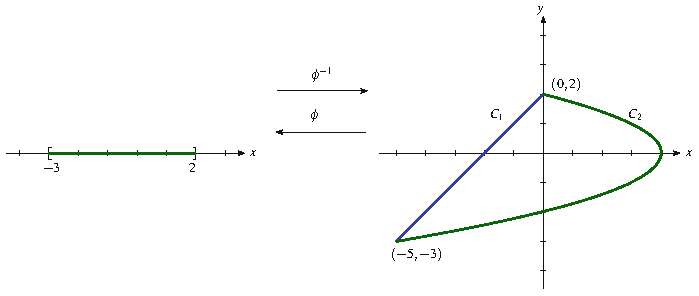
\includegraphics[width=0.945\linewidth]{images/vector/fig-7-16.pdf}
  \caption{映射 $\varphi^{-1}$ 把 $[-3,2]$ 送到曲线 $C_2$}
  \label{fig:7-16}
\end{figure}

\textbf{例二.} 在这个例子中，我们将做一些与例一中类似的事情. 回想在例一中，我们沿两条具有相同起点和终点的不同曲线 $C_1$ 和 $C_2$ 积分了一个 1-形式，并发现这两个积分是不同的，也就是说，积分依赖于所取的路径. 我们将使用一个不同的 1-形式来重复这一点. 这次我们积分的 1-形式将是一种特殊的 1-形式，它将是某个 0-形式的外微分.

我们将选择 $\mathbb{R}^2$ 上的 0-形式（函数）$f(x,y)=x^2y$. 对这个 0-形式取外微分，给出 1-形式
\[
df=\frac{\partial f}{\partial x}dx+\frac{\partial f}{\partial y}dy=2xy\,dx+x^2dy.
\]
这就是我们要积分的 1-形式. 我们将使用与例一中相同的路径和参数化. 这个过程本质上与前面的例子相同. 我们知道 $T^*\varphi^{-1}\cdot\bigl(2xydx+x^2dy\bigr)$ 是 $\mathbb{R}$ 上的 1-形式，所以它必然具有某个函数 $f(t)$ 决定的 $f(t)\,dt$ 的形式. 对曲线 $C_1$，我们求出
\begin{align*}
f(t)&=f(t)\,dt\bigl([1]\bigr)\\
&=T^*\varphi^{-1}\cdot\bigl(2xydx+x^2dy\bigr)\bigl([1]\bigr)\\
&=\bigl(2xydx+x^2dy\bigr)\binom{5}{5}\\
&=10xy+5x^2\\
&=10(5t-5)(5t-3)+5(5t-5)^2\\
&=5(75t^2-130t+55),
\end{align*}
于是我们有 $T^*\varphi^{-1}\cdot\bigl(2xydx+x^2dy\bigr)=5(75t^2-130t+55)\,dt$. 我们使用恒等式 $\int_C\alpha=\int_{\varphi(C)}T^*\varphi^{-1}\cdot\alpha$，得到
\begin{align*}
\int_{C_1}2xydx+x^2dy
&=\int_{\varphi(C_1)}T^*\varphi^{-1}\cdot\bigl(2xydx+x^2dy\bigr)\\
&=\int_{[0,1]}5(75t^2-130t+55)\,dt\\
&=75.
\end{align*}
现在我们沿路径 $C_2$ 取积分. 类似地我们求出
\begin{align*}
f(t)&=f(t)\,dt\bigl([1]\bigr)\\
&=T^*\varphi^{-1}\cdot\bigl(2xydx+x^2dy\bigr)\bigl([1]\bigr)\\
&=\bigl(2xydx+x^2dy\bigr)\binom{-2t}{1}\\
&=2xy(-2t)+x^2(1)\\
&=2(4-t^2)(t)(-2t)+(4-t^2)^2\\
&=5t^4-24t^2+16,
\end{align*}
于是我们有 $T^*\varphi^{-1}\cdot\bigl(2xydx+x^2dy\bigr)=\bigl(5t^4-24t^2+16\bigr)dt$. 积分是
\begin{align*}
\int_{C_2}2xydx+x^2dy
&=\int_{\varphi(C_2)}T^*\varphi^{-1}\cdot\bigl(2xydx+x^2dy\bigr)\\
&=\int_{[-3,2]}\bigl(5t^4-24t^2+16\bigr)dt\\
&=75.
\end{align*}
有趣的事情发生了. 当我们的 1-形式是某个 0-形式的外微分时，我们的积分结果似乎不依赖于所取的路径. 事实上，这普遍成立，并不仅仅在这个例子中成立. 我们将在后面更详细地考察这一点.

\textbf{例三.} 我们的下一个例子涉及在 $\mathbb{R}^3$ 中沿从点 $(2,0,0)$ 到点 $(3,4,5)$ 的直线路径 $C$ 积分 1-形式 $ydx+zdy+xdz$. 我们求这条路径的一个参数化 $\varphi^{-1}:\mathbb{R}\to\mathbb{R}^3$，由 $\varphi^{-1}(t)=\bigl(x(t),y(t),z(t)\bigr)=(2+t,4t,5t)$ 给出. 令 $R=[0,1]\subset\mathbb{R}$，我们有 $\varphi^{-1}(R)=\bigl\{(x,y,z)\,\bigl|\,x=2+t,\ y=4t,\ z=5t,\ 0\leq t\leq 1\bigr\}=C$. 这给出
\[
T_p\varphi^{-1}=\begin{bmatrix}\frac{\partial x}{\partial t}\\\frac{\partial y}{\partial t}\\\frac{\partial z}{\partial t}\end{bmatrix}_p=\begin{bmatrix}1\\4\\5\end{bmatrix}.
\]
显然，$T_p\varphi^{-1}$ 不依赖于基点 $p\in\mathbb{R}$. 和之前一样，我们知道 $T^*\varphi^{-1}\cdot(ydx+zdy+xdz)=f(t)\,dt$，其中 $f(t)$ 是某个函数，正是我们想求的. 计算过程与之前完全相同，
\begin{align*}
f(t)&=f(t)\,dt\bigl([1]\bigr)\\
&=T^*\varphi^{-1}\cdot(ydx+zdy+xdz)\bigl([1]\bigr)\\
&=(ydx+zdy+xdz)\bigl(T\varphi^{-1}\cdot[1]\bigr)\\
&=(ydx+zdy+xdz)\begin{bmatrix}1\\4\\5\end{bmatrix}\cdot[1]\\
&=ydx\begin{bmatrix}1\\4\\5\end{bmatrix}+zdy\begin{bmatrix}1\\4\\5\end{bmatrix}+xdz\begin{bmatrix}1\\4\\5\end{bmatrix}\\
&=y(1)+z(4)+x(5)\\
&=(4t)+4(5t)+5(2+t)\\
&=29t+10,
\end{align*}
于是我们有 $T^*\varphi^{-1}\cdot(ydx+zdy+xdz)=(29t+10)dt$. 利用 $\int_C\alpha=\int_{\varphi(C)}T^*\varphi^{-1}\cdot\alpha$，我们得到积分
\begin{align*}
\int_C(ydx+zdy+xdz)
&=\int_{\varphi(C)}T^*\varphi^{-1}\cdot(ydx+zdy+xdz)\\
&=\int_{[0,1]}(29t+10)\,dt\\
&=24\frac{1}{2}.
\end{align*}

\subsection{曲面积分}

现在我们将做几个在参数化二维曲面上积分 2-形式的例子.

\textbf{例一.} 我们将在单位球面的上半部分上积分 2-形式 $z^2dx\wedge dy$. 我们将使用由
\[
\varphi^{-1}(r,\theta)=\bigl(x(r,\theta),y(r,\theta),z(r,\theta)\bigr)=\Bigl(r\cos\theta,\ r\sin\theta,\ \sqrt{1-r^2}\Bigr)
\]
给出的参数化. 令 $R=\bigl\{(r,\theta)\,\bigl|\,0\leq r\leq 1,\ 0\leq\theta\leq 2\pi\bigr\}$，我们有 $\varphi^{-1}(R)$ 是单位球面的上半部分. 见图~\ref{fig:7-17}. 首先我们求 $T\varphi^{-1}$，
\begin{align*}
T\varphi^{-1}&=\begin{bmatrix}\frac{\partial x}{\partial r}&\frac{\partial x}{\partial\theta}\\\frac{\partial y}{\partial r}&\frac{\partial y}{\partial\theta}\\\frac{\partial z}{\partial r}&\frac{\partial z}{\partial\theta}\end{bmatrix}
=\begin{bmatrix}\frac{\partial(r\cos\theta)}{\partial r}&\frac{\partial(r\cos\theta)}{\partial\theta}\\\frac{\partial(r\sin\theta)}{\partial r}&\frac{\partial(r\sin\theta)}{\partial\theta}\\\frac{\partial\sqrt{1-r^2}}{\partial r}&\frac{\partial\sqrt{1-r^2}}{\partial\theta}\end{bmatrix}\\
&=\begin{bmatrix}\cos\theta&-r\sin\theta\\\sin\theta&r\cos\theta\\-\frac{r}{\sqrt{1-r^2}}&0\end{bmatrix}.
\end{align*}

\begin{figure}[htbp]
  \centering
  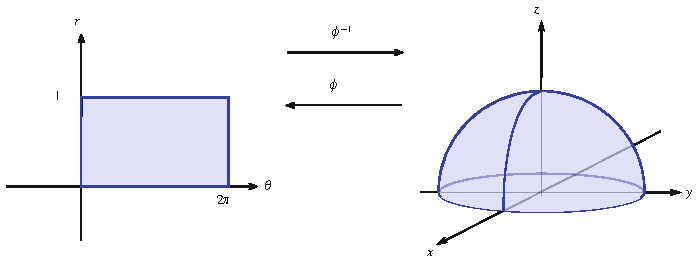
\includegraphics[width=0.957\linewidth]{images/vector/fig-7-17.pdf}
  \caption{映射 $\varphi^{-1}$ 把 $R=\bigl\{(r,\theta)\,\bigl|\,0\leq r\leq 1,\ 0\leq\theta\leq 2\pi\bigr\}$ 送到 $\mathbb{R}^3$ 中单位球面的顶部}
  \label{fig:7-17}
\end{figure}

现在我们要求 $T^*\varphi^{-1}\cdot\bigl(z^2dx\wedge dy\bigr)$. 我们知道这是 $\mathbb{R}^2$ 上的 2-形式，所以它必然具有某个函数 $g(r,\theta)$ 决定的 $g(r,\theta)\,dr\wedge d\theta$ 的形式. 我们的目标是求出这个函数. 注意
\[
g(r,\theta)\,dr\wedge d\theta\left(\binom{1}{0},\binom{0}{1}\right)=g(r,\theta)\begin{vmatrix}1&0\\0&1\end{vmatrix}=g(r,\theta).
\]
因此，
\begin{align*}
g(r,\theta)&=g(r,\theta)\,dr\wedge d\theta\left(\binom{1}{0},\binom{0}{1}\right)\\
&=T^*\varphi^{-1}\cdot\bigl(z^2dx\wedge dy\bigr)\left(\binom{1}{0},\binom{0}{1}\right)\\
&=z^2dx\wedge dy\left(T\varphi^{-1}\cdot\binom{1}{0},T\varphi^{-1}\cdot\binom{0}{1}\right)\\
&=z^2dx\wedge dy\left(\begin{bmatrix}\cos\theta\\\sin\theta\\-\frac{r}{\sqrt{1-r^2}}\end{bmatrix},\begin{bmatrix}-r\sin\theta\\r\cos\theta\\0\end{bmatrix}\right)\\
&=z^2\begin{vmatrix}\cos\theta&-r\sin\theta\\\sin\theta&r\cos\theta\end{vmatrix}\\
&=z^2r\\
&=\Bigl(\sqrt{1-r^2}\Bigr)^2r\\
&=r-r^3,
\end{align*}
\[
\Rightarrow\ T^*\varphi^{-1}\cdot\bigl(z^2dx\wedge dy\bigr)=\bigl(r-r^3\bigr)dr\wedge d\theta.
\]
利用恒等式 $\int_R\alpha=\int_{\varphi(R)}T^*\varphi^{-1}\cdot\alpha$，我们有
\begin{align*}
\int_R z^2dx\wedge dy
&=\int_{\varphi(R)}\bigl(r-r^3\bigr)dr\wedge d\theta\\
&=\int_0^{2\pi}\int_0^1\bigl(r-r^3\bigr)dr\,d\theta\\
&=\int_0^{2\pi}\left.\left(\frac{r^2}{2}-\frac{r^4}{4}\right)\right|_0^1d\theta\\
&=\int_0^{2\pi}\frac{1}{4}\,d\theta\\
&=\frac{\pi}{2}.
\end{align*}

\textbf{例二.} 现在我们将使用下面三种参数化，在单位球面的上半部分上积分 2-形式 $\alpha=\frac{1}{x}dy\wedge dz-\frac{1}{y}dx\wedge dz$. 我们将完成第一个参数化，把另外两个留作练习.
\begin{enumerate}
  \item[(a)] $(r,\theta)\mapsto\Bigl(r\cos\theta,\ r\sin\theta,\ \sqrt{1-r^2}\Bigr)$，$0\leq\theta\leq 2\pi$，$0\leq r\leq 1$
  \item[(b)] $(\theta,\varphi)\mapsto(\sin\varphi\cos\theta,\ \sin\varphi\sin\theta,\ \cos\varphi)$，$0\leq\theta\leq 2\pi$，$0\leq\varphi\leq\frac{\pi}{2}$
  \item[(c)] $(x,y)\mapsto\Bigl(x,\ y,\ \sqrt{1-x^2-y^2}\Bigr)$，$x^2+y^2\leq 1$
\end{enumerate}
我们应该预期，无论使用哪种参数化，都会得到相同的答案. 我们现在进行第一个参数化，它仿照例一，只不过我们有
\[
g(r,\theta)\,dr\wedge d\theta=T^*\varphi^{-1}\cdot\left(\frac{1}{x}dy\wedge dz-\frac{1}{y}dx\wedge dz\right)\longmapsto\frac{1}{x}dy\wedge dz-\frac{1}{y}dx\wedge dz.
\]
我们想求 $g(r,\theta)$，令 $e_1$ 和 $e_2$ 分别是 $r$ 方向和 $\theta$ 方向的单位向量，于是我们有
\begin{align*}
g(r,\theta)&=g(r,\theta)\,dr\wedge d\theta(e_1,e_2)\\
&=T^*\varphi^{-1}\cdot\left(\frac{1}{x}dy\wedge dz-\frac{1}{y}dx\wedge dz\right)(e_1,e_2)\\
&=\left(\frac{1}{x}dy\wedge dz-\frac{1}{y}dx\wedge dz\right)(T\varphi\cdot e_1,T\varphi\cdot e_2)\\
&=\left(\frac{1}{x}dy\wedge dz-\frac{1}{y}dx\wedge dz\right)\left(\begin{bmatrix}\cos\theta\\\sin\theta\\-\frac{r}{\sqrt{1-r^2}}\end{bmatrix},\begin{bmatrix}-r\sin\theta\\r\cos\theta\\0\end{bmatrix}\right)\\
&=\frac{1}{x}dy\wedge dz\left(\begin{bmatrix}\cos\theta\\\sin\theta\\-\frac{r}{\sqrt{1-r^2}}\end{bmatrix},\begin{bmatrix}-r\sin\theta\\r\cos\theta\\0\end{bmatrix}\right)-\frac{1}{y}dx\wedge dz\left(\begin{bmatrix}\cos\theta\\\sin\theta\\-\frac{r}{\sqrt{1-r^2}}\end{bmatrix},\begin{bmatrix}-r\sin\theta\\r\cos\theta\\0\end{bmatrix}\right)\\
&=\frac{1}{x}\begin{vmatrix}\sin\theta&r\cos\theta\\-\frac{r}{\sqrt{1-r^2}}&0\end{vmatrix}-\frac{1}{y}\begin{vmatrix}\cos\theta&-r\sin\theta\\-\frac{r}{\sqrt{1-r^2}}&0\end{vmatrix}\\
&=\frac{1}{x}\frac{r^2\cos\theta}{\sqrt{1-r^2}}-\frac{1}{y}\frac{-r^2\sin\theta}{\sqrt{1-r^2}}\\
&=\frac{1}{r\cos\theta}\frac{r^2\cos\theta}{\sqrt{1-r^2}}-\frac{1}{r\sin\theta}\frac{-r^2\sin\theta}{\sqrt{1-r^2}}\\
&=\frac{2r}{\sqrt{1-r^2}},
\end{align*}
\[
\Rightarrow\ T^*\varphi^{-1}\cdot\left(\frac{1}{x}dy\wedge dz-\frac{1}{y}dx\wedge dz\right)=\frac{2r}{\sqrt{1-r^2}}dr\wedge d\theta.
\]
现在我们用恒等式 $\int_R\alpha=\int_{\varphi(R)}T^*\varphi^{-1}\cdot\alpha$ 来取积分，
\begin{align*}
\int_R\frac{1}{x}dy\wedge dz-\frac{1}{y}dx\wedge dz
&=\int_{\varphi(R)}\frac{2r}{\sqrt{1-r^2}}dr\wedge d\theta\\
&=\int_0^{2\pi}\int_0^1\frac{2r}{\sqrt{1-r^2}}dr\,d\theta\\
&=2\int_0^{2\pi}d\theta\cdot\int_0^1\frac{r}{\sqrt{1-r^2}}dr\\
&=2\cdot 2\pi\cdot\left[-\sqrt{1-r^2}\right]_0^1\\
&=4\pi.
\end{align*}

\begin{question}\label{q:7-13}
用第二种和第三种参数化求积分，完成这个例子.
\end{question}

\section{小结、参考文献与问题}

\subsection{小结}

如果求积分 $\int_R f(x_1,x_2,\ldots,x_n)\,dx_1dx_2\cdots dx_n$ 是困难的，但通过做变量替换
\[
\mathbb{R}^n_{x_1x_2\cdots x_n}\xrightarrow{\ \varphi\ }\mathbb{R}^n_{\varphi_1\varphi_2\cdots\varphi_n},\qquad(x_1,x_2,\ldots,x_n)\longmapsto(\varphi_1,\varphi_2,\ldots,\varphi_n)
\]
它会变得容易，那么就可以使用变量替换公式
\[
\begin{aligned}
\text{变量替换公式}\qquad \int_R f(x_1,\ldots,x_n)\,dx_1\wedge\cdots\wedge dx_n
&=\int_{\varphi(R)}f\circ\varphi^{-1}(\varphi_1,\ldots,\varphi_n)\,T^*\varphi^{-1}\\
&\quad\cdot\bigl(dx_1\wedge\cdots\wedge dx_n\bigr).
\end{aligned}
\]
左边在 $x_1\cdots x_n$-坐标中进行，我们在区域 $R$ 上用与 $x_1\cdots x_n$-坐标相联系的体积形式 $dx_1\wedge\cdots\wedge dx_n$ 积分函数 $f(x_1,\ldots,x_n)$. 在右边，函数 $f\circ\varphi^{-1}:\mathbb{R}^n\to\mathbb{R}$ 是变量 $\varphi_1,\varphi_2,\ldots,\varphi_n$ 的函数. 我们在 $\mathbb{R}^n_{\varphi_1\varphi_2\cdots\varphi_n}$ 中积分的区域是像 $\varphi(R)$. 最后，右边的形式是 $T^*\varphi^{-1}\cdot\bigl(dx_1\wedge\cdots\wedge dx_n\bigr)$，即面积形式 $dx_1\wedge\cdots\wedge dx_n$ 由 $\varphi^{-1}$ 的拉回，而不是面积形式 $d\varphi_1\wedge\cdots\wedge d\varphi_n$. 这恰好给出了你在多元微积分中使用极坐标、柱坐标和球坐标做变量替换时用到的东西.

我们可以在曲线上积分 1-形式，在曲面上积分 2-形式，在三维空间中积分 3-形式，等等. 只要在一个 $n$ 维流形上有一个 $n$-形式，我们就可以对它积分. 给定流形 $\Sigma_k\subset\mathbb{R}^n$（$k<n$）的一个参数化，即一个可逆映射 $\varphi^{-1}:U\subset\mathbb{R}^k\to\Sigma_k\subset\mathbb{R}^n$，我们可以把 $k$-形式拉回到 $U\subset\mathbb{R}^k$ 并在那里积分，从而在 $\Sigma_k$ 上积分 $k$-形式. 在这种情况下，我们想使用的变量替换公式的版本是
\[
\text{$k$ 维参数化曲面 $\Sigma_k$ 上 $k$-形式的积分}\qquad\int_{\Sigma_k}\alpha=\int_{\varphi(\Sigma_k)}T^*\varphi^{-1}\cdot\alpha.
\]
当 $k=1$ 时，我们得到一条曲线，经常写 $\Sigma_1=C$；当 $k=2$ 时，我们得到一个曲面，经常写 $\Sigma_2=S$；当 $k=3$ 时，我们得到一个体积，经常写 $\Sigma_3=V$.

\subsection{参考文献与进一步阅读}

Riemann 和与变量替换几乎在每一本微积分或入门分析书中都会引入并讨论，而且常常不惜篇幅，例如见 Steward~\cite{ref43}、Hubbard 与 Hubbard~\cite{ref27}，或 Marsden 与 Hoffman~\cite{ref31}. 然而，在本章中，我们大体上遵循了 Bachman~\cite{ref04} 的讲述，因为它直接涉及微分形式的情形. 关于同一材料的更偏理论性的导引，另见 Watschap~\cite{ref47} 或 Renteln~\cite{ref37}.

\subsection{问题}

\begin{question}\label{q:7-14}
设 $C$ 是 $\mathbb{R}^3$ 中由 $\gamma(t)=\bigl(2t+1,\ t^2,\ t^3\bigr)$（$1\leq t\leq 3$）参数化的定向曲线，设 $\alpha=(3x-1)^2dx+5dy+2dz$ 是 $\mathbb{R}^3$ 上的 1-形式. 求 $\int_C\alpha$.
\end{question}

\begin{question}\label{q:7-15}
设 $C$ 是 $\mathbb{R}^3$ 中由 $\gamma(t)=\bigl(1-t^2,\ t^3-t,\ 0\bigr)$（$0\leq t\leq 2$）参数化的定向曲线. 注意曲线 $C$ 位于 $\mathbb{R}^2\subset\mathbb{R}^3$ 中. 设 $\alpha=-5xy\,dx+dz$ 是 $\mathbb{R}^3$ 上的 1-形式. 求 $\int_C\alpha$.
\end{question}

\begin{question}\label{q:7-16}
设 $C$ 是 $\mathbb{R}^2$ 中由 $\gamma(t)=\bigl(t^2,\ 2t+1\bigr)$（$1\leq t\leq 2$）参数化的曲线，设 $\alpha=4x\,dx+ydy$ 是 $\mathbb{R}^2$ 上的 1-形式. 求 $\int_C\alpha$.
\end{question}

\begin{question}\label{q:7-17}
设 $C$ 是平面 $\mathbb{R}^2$ 中作为函数 $y=1+x^2$（$-1\leq x\leq 1$）图像的曲线，按 $x$ 增大的方向定向，设 $\alpha=y\,dx+x\,dy$ 是平面上的 1-形式. 求 $\int_C\alpha$. （虽然并非必要，也可以把曲线 $C$ 参数化为 $\gamma(t)=(t,1+t^2)$，$-1\leq t\leq 1$.）
\end{question}

\begin{question}\label{q:7-18}
设 $C_1$ 和 $C_2$ 是平面 $\mathbb{R}^2$ 中的曲线，分别由 $\gamma_1(t)=(t-1,2t-1)$（$1\leq t\leq 2$）和 $\gamma_2(u)=(2-u,5-2u)$（$1\leq u\leq 2$）参数化. 设 $\alpha=y\,dx$ 是 $\mathbb{R}^2$ 上的 1-形式. 求 $\int_{C_1}\alpha$ 和 $\int_{C_2}\alpha$. 比较这两个答案，并解释它们之间的关系.
\end{question}

\begin{question}\label{q:7-19}
设 $C$ 是 $\mathbb{R}^2$ 中由 $\gamma(\theta)=\bigl(\cos(\theta),\sin(\theta)\bigr)$（$0\leq\theta\leq 2\pi$）参数化的单位圆. 设
\[
\alpha_1=\frac{-y}{x^2+y^2}dx+\frac{x}{x^2+y^2}dy,\qquad
\alpha_2=\frac{x}{x^2+y^2}dx+\frac{y}{x^2+y^2}dy
\]
是 $\mathbb{R}^2$ 上的 1-形式. 求 $\int_C\alpha_1$ 和 $\int_C\alpha_2$. 注意，可以把 $\alpha_1$ 写成 $\alpha_1=-\sin(\theta)\,dx+\cos(\theta)\,dy$，把 $\alpha_2$ 写成 $\alpha_2=\cos(\theta)\,dx+\sin(\theta)\,dy$.
\end{question}

\begin{question}\label{q:7-20}
设 $C$ 是 $\mathbb{R}^2$ 中的一条曲线. 曲线 $C$ 既可以由 $\gamma_1(t)=\bigl(t,\sqrt{1+t^2}\bigr)$（$-1\leq t\leq 1$）参数化，也可以由 $\gamma_2(\theta)=\bigl(\tan(\theta),\sec(\theta)\bigr)$（$-\frac{\pi}{4}\leq\theta\leq\frac{\pi}{4}$）参数化. 设 $\alpha=y^2\,dx$ 是 $\mathbb{R}^2$ 上的 1-形式. 用 $C$ 的每一种参数化求 $\int_C\alpha$.
\end{question}

\begin{question}\label{q:7-21}
设 $C$ 是 $\mathbb{R}^2$ 中的一条曲线. 曲线 $C$ 可以参数化为 $\gamma_1(t)=\bigl(t,t^2\bigr)$（$-2\leq t\leq 2$），或者 $\gamma_2(u)=\bigl(u^3+u,\ u^6+2u^4+u^2\bigr)$（$-1\leq u\leq 1$），或者 $\gamma_3(\theta)=\bigl(4\sin(\theta),\ 16\sin^2(\theta)\bigr)$（$-\frac{\pi}{6}\leq\theta\leq\frac{\pi}{6}$）. 如果 $\alpha=5xy\,dy$ 是 $\mathbb{R}^2$ 上的 1-形式，用全部三种参数化求 $\int_C\alpha$.
\end{question}

\begin{question}\label{q:7-22}
考虑 $\mathbb{R}^3$ 中由 $\varphi(x,y)=\bigl(x,\ y,\ x^3+xy^2\bigr)$（$1\leq x\leq 3,\ 1\leq y\leq 2$）参数化的曲面 $S$，以及 $\mathbb{R}^3$ 上的 2-形式 $\beta=2xyz\,dx\wedge dy+6(2x^3-y^3)\,dy\wedge dz+z\,dz\wedge dx$. 求 $\int_S\beta$.
\end{question}

\begin{question}\label{q:7-23}
设 $U$ 是单位圆盘的上半部分，$U=\bigl\{(x,y)\,\bigl|\,-1\leq x\leq 1,\ 0\leq y\leq\sqrt{1-x^2}\bigr\}$. 设 $\mathbb{R}^3$ 中的曲面 $S$ 由 $\varphi(x,y)=\bigl(x,\ y,\ x^2+y^2\bigr)$（$(x,y)\in U$）参数化，设 $\beta=6y\,dx\wedge dy$ 是 $\mathbb{R}^3$ 上的 2-形式. 求 $\int_S\beta$.
\end{question}

\begin{question}\label{q:7-24}
设 $U$ 是 $\mathbb{R}^2$ 中的三角形区域 $U=\bigl\{(u,v)\,\bigl|\,0\leq u\leq 1,\ 0\leq v\leq 1-u\bigr\}$. 设 $\mathbb{R}^3$ 中的曲面 $S$ 由 $\varphi(u,v)=\bigl(u-v,\ uv,\ u^2+(v+1)^2\bigr)$（$(u,v)\in U$）参数化，设 $\beta=-(1+x^2)\,dx\wedge dy+dy\wedge dz$. 求 $\int_S\beta$.
\end{question}

\begin{question}\label{q:7-25}
设 $U=\bigl\{(u,v)\,\bigl|\,-1\leq u\leq 1,\ -2\leq v\leq 2\bigr\}\subset\mathbb{R}^2$，设 $\mathbb{R}^3$ 中的曲面 $S$ 由 $\varphi(u,v)=\bigl(u,\ v,\ u^3+3uv^2\bigr)$（$(u,v)\in U$）参数化. 设 $\beta=-dy\wedge dz+dz\wedge dx$. 求 $\int_S\beta$.
\end{question}

\begin{question}\label{q:7-26}
设 $U=\bigl\{(u,v)\,\bigl|\,0\leq u\leq 1,\ 0\leq v\leq 2\bigr\}\subset\mathbb{R}^2$，设 $\mathbb{R}^3$ 中的曲面 $S$ 由 $\varphi(u,v)=\bigl(u,\ v,\ u^2+v^3\bigr)$（$(u,v)\in U$）参数化. 设 $\beta=31x^2y^3\,dx\wedge dy+5xz\,dy\wedge dz+7yz\,dz\wedge dx$. 求 $\int_S\beta$.
\end{question}

\begin{question}\label{q:7-27}
设 $U=\bigl\{(u,v)\,\bigl|\,u^2+v^2\leq 9\bigr\}\subset\mathbb{R}^2$，设 $\mathbb{R}^3$ 中的曲面 $S$ 由 $\varphi(u,v)=\bigl(u,\ v,\ 7+(u^2+v^2)\bigr)$（$(u,v)\in U$）参数化. 设 $\beta=z^2dx\wedge dy$. 求 $\int_S\beta$.
\end{question}

\begin{question}\label{q:7-28}
设 $U=\bigl\{(u,v)\,\bigl|\,u^2+v^2\leq 9\bigr\}\subset\mathbb{R}^2$，设 $\mathbb{R}^3$ 中的曲面 $S$ 由 $\varphi(u,v)=\bigl(u,\ v,\ 25-(u^2+v^2)\bigr)$（$(u,v)\in U$）参数化. 设 $\beta=z^2dx\wedge dy$. 求 $\int_S\beta$.
\end{question}

\begin{question}\label{q:7-29}
设 $U=\bigl\{(u,v)\,\bigl|\,0\leq u\leq 1,\ 0\leq v\leq 2\bigr\}\subset\mathbb{R}^2$，设 $\mathbb{R}^3$ 中的曲面 $S$ 由 $\varphi(u,v)=\bigl(u+v,\ u-v^2,\ uv\bigr)$（$(u,v)\in U$）参数化. 设 $\beta=6z\,dz\wedge dx$. 求 $\int_S\beta$.
\end{question}

\begin{question}\label{q:7-30}
设 $U=\bigl\{(u,v)\,\bigl|\,1\leq u\leq 2,\ 0\leq v\leq 2\pi\bigr\}\subset\mathbb{R}^2$，设 $\mathbb{R}^3$ 中的曲面 $S$ 由 $\varphi(u,v)=\bigl(u^3\cos(v),\ u^3\sin(v),\ u^2\bigr)$（$(u,v)\in U$）参数化. 设 $\beta=2z\,dx\wedge dy-x\,dy\wedge dz-y\,dz\wedge dx$. 求 $\int_S\beta$.
\end{question}

\begin{question}\label{q:7-31}
设 $\alpha=xy\,dx\wedge dy$ 是 $\mathbb{R}^2$ 上的 2-形式，设 $D$ 是以原点为圆心、半径为 3 的圆盘. 用极坐标变量替换求 $\int_D\alpha$.
\end{question}

\begin{question}\label{q:7-32}
设 $\alpha=(3x+4y^2)\,dx\wedge dy$ 是 $\mathbb{R}^2$ 上的 2-形式，设 $R$ 是由圆 $x^2+y^2=1$ 和 $x^2+y^2=9$ 围成的上半平面中的区域. 用极坐标变量替换求 $\int_R\alpha$.
\end{question}

\begin{question}\label{q:7-33}
设 $\alpha=(x+y)\,dx\wedge dy$ 是 $\mathbb{R}^2$ 上的 2-形式，设 $R$ 是 $y$ 轴左侧、由圆 $x^2+y^2=1$ 和 $x^2+y^2=9$ 围成的区域. 用极坐标变量替换求 $\int_R\alpha$.
\end{question}

\begin{question}\label{q:7-34}
设 $\alpha=\cos(x^2+y^2)\,dx\wedge dy$ 是 $\mathbb{R}^2$ 上的 2-形式，设 $R$ 是 $x$ 轴上方、圆 $x^2+y^2=4$ 内部的区域. 用极坐标变量替换求 $\int_R\alpha$.
\end{question}

\begin{question}\label{q:7-35}
设 $V\subset\mathbb{R}^3$ 是位于圆柱面 $x^2+y^2=1$ 内部、平面 $z=0$ 与 $z=5$ 之间的区域，设 $\beta=x\,dx\wedge dy\wedge dz$ 是 $\mathbb{R}^3$ 上的 3-形式. 用柱坐标变量替换求 $\int_V\beta$.
\end{question}

\begin{question}\label{q:7-36}
设 $V\subset\mathbb{R}^3$ 是位于圆柱面 $x^2+y^2=25$ 内部、平面 $z=-5$ 与 $z=5$ 之间的区域，设 $\beta=\sqrt{x^2+y^2}\,dx\wedge dy\wedge dz$ 是 $\mathbb{R}^3$ 上的 3-形式. 用柱坐标变量替换求 $\int_V\beta$.
\end{question}

\begin{question}\label{q:7-37}
设 $V=\Bigl\{(x,y,z)\,\Bigl|\,-2\leq x\leq 2,\ -\sqrt{4-x^2}\leq y\leq\sqrt{4-x^2},\ \sqrt{x^2+y^2}\leq z\leq 2\Bigr\}\subset\mathbb{R}^3$，设 $\beta=(x^2+y^2)\,dx\wedge dy\wedge dz$ 是 $\mathbb{R}^3$ 上的 3-形式. 用柱坐标变量替换求 $\int_V\beta$.
\end{question}

\begin{question}\label{q:7-38}
设 $V\subset\mathbb{R}^3$ 是位于圆柱面 $x^2+y^2=1$ 与 $x^2+y^2=4$ 之间、平面 $z=0$ 与 $z=x+2$ 之间的区域，设 $\beta=y\,dx\wedge dy\wedge dz$ 是 $\mathbb{R}^3$ 上的 3-形式. 用柱坐标变量替换求 $\int_V\beta$.
\end{question}

\begin{question}\label{q:7-39}
设 $V=\bigl\{(x,y,z)\,\bigl|\,x^2+y^2+z^2\leq 1\bigr\}$，即 $\mathbb{R}^3$ 中的单位球，设 $\beta=e^{(x^2+y^2+z^2)^{3/2}}dx\wedge dy\wedge dz$ 是 $\mathbb{R}^3$ 上的 3-形式. 用球坐标变量替换求 $\int_V\beta$.
\end{question}

\begin{question}\label{q:7-40}
设 $V=\bigl\{(x,y,z)\,\bigl|\,x^2+y^2+z^2\leq 1\bigr\}$，即 $\mathbb{R}^3$ 中的单位球，设 $\beta=e^{(x^2+y^2+z^2)^{3/2}}dx\wedge dy\wedge dz$ 是 $\mathbb{R}^3$ 上的 3-形式. 用球坐标变量替换求 $\int_V\beta$.
\end{question}

\begin{question}\label{q:7-41}
设 $V=\bigl\{(x,y,z)\,\bigl|\,x^2+y^2+z^2\leq 5\bigr\}$，即以原点为球心、半径为 $\sqrt{5}$ 的球，设 $\beta=(x^2+y^2+z^2)^2\,dx\wedge dy\wedge dz$ 是 $\mathbb{R}^3$ 上的 3-形式. 用球坐标变量替换求 $\int_V\beta$.
\end{question}

\begin{question}\label{q:7-42}
求 $\mathbb{R}^3$ 中圆锥面 $z=\sqrt{x^2+y^2}$ 上方、球面 $x^2+y^2+z^2=z$ 下方的区域的体积. 这意味着我们要积分的 3-形式是体积形式 $dx\wedge dy\wedge dz$. 使用球坐标变量替换.
\end{question}
